% Options for packages loaded elsewhere
\PassOptionsToPackage{unicode}{hyperref}
\PassOptionsToPackage{hyphens}{url}
\documentclass[
]{article}
\usepackage{xcolor}
\usepackage[margin=1in]{geometry}
\usepackage{amsmath,amssymb}
\setcounter{secnumdepth}{5}
\usepackage{iftex}
\ifPDFTeX
  \usepackage[T1]{fontenc}
  \usepackage[utf8]{inputenc}
  \usepackage{textcomp} % provide euro and other symbols
\else % if luatex or xetex
  \usepackage{unicode-math} % this also loads fontspec
  \defaultfontfeatures{Scale=MatchLowercase}
  \defaultfontfeatures[\rmfamily]{Ligatures=TeX,Scale=1}
\fi
\usepackage{lmodern}
\ifPDFTeX\else
  % xetex/luatex font selection
\fi
% Use upquote if available, for straight quotes in verbatim environments
\IfFileExists{upquote.sty}{\usepackage{upquote}}{}
\IfFileExists{microtype.sty}{% use microtype if available
  \usepackage[]{microtype}
  \UseMicrotypeSet[protrusion]{basicmath} % disable protrusion for tt fonts
}{}
\makeatletter
\@ifundefined{KOMAClassName}{% if non-KOMA class
  \IfFileExists{parskip.sty}{%
    \usepackage{parskip}
  }{% else
    \setlength{\parindent}{0pt}
    \setlength{\parskip}{6pt plus 2pt minus 1pt}}
}{% if KOMA class
  \KOMAoptions{parskip=half}}
\makeatother
\usepackage{color}
\usepackage{fancyvrb}
\newcommand{\VerbBar}{|}
\newcommand{\VERB}{\Verb[commandchars=\\\{\}]}
\DefineVerbatimEnvironment{Highlighting}{Verbatim}{commandchars=\\\{\}}
% Add ',fontsize=\small' for more characters per line
\usepackage{framed}
\definecolor{shadecolor}{RGB}{248,248,248}
\newenvironment{Shaded}{\begin{snugshade}}{\end{snugshade}}
\newcommand{\AlertTok}[1]{\textcolor[rgb]{0.94,0.16,0.16}{#1}}
\newcommand{\AnnotationTok}[1]{\textcolor[rgb]{0.56,0.35,0.01}{\textbf{\textit{#1}}}}
\newcommand{\AttributeTok}[1]{\textcolor[rgb]{0.13,0.29,0.53}{#1}}
\newcommand{\BaseNTok}[1]{\textcolor[rgb]{0.00,0.00,0.81}{#1}}
\newcommand{\BuiltInTok}[1]{#1}
\newcommand{\CharTok}[1]{\textcolor[rgb]{0.31,0.60,0.02}{#1}}
\newcommand{\CommentTok}[1]{\textcolor[rgb]{0.56,0.35,0.01}{\textit{#1}}}
\newcommand{\CommentVarTok}[1]{\textcolor[rgb]{0.56,0.35,0.01}{\textbf{\textit{#1}}}}
\newcommand{\ConstantTok}[1]{\textcolor[rgb]{0.56,0.35,0.01}{#1}}
\newcommand{\ControlFlowTok}[1]{\textcolor[rgb]{0.13,0.29,0.53}{\textbf{#1}}}
\newcommand{\DataTypeTok}[1]{\textcolor[rgb]{0.13,0.29,0.53}{#1}}
\newcommand{\DecValTok}[1]{\textcolor[rgb]{0.00,0.00,0.81}{#1}}
\newcommand{\DocumentationTok}[1]{\textcolor[rgb]{0.56,0.35,0.01}{\textbf{\textit{#1}}}}
\newcommand{\ErrorTok}[1]{\textcolor[rgb]{0.64,0.00,0.00}{\textbf{#1}}}
\newcommand{\ExtensionTok}[1]{#1}
\newcommand{\FloatTok}[1]{\textcolor[rgb]{0.00,0.00,0.81}{#1}}
\newcommand{\FunctionTok}[1]{\textcolor[rgb]{0.13,0.29,0.53}{\textbf{#1}}}
\newcommand{\ImportTok}[1]{#1}
\newcommand{\InformationTok}[1]{\textcolor[rgb]{0.56,0.35,0.01}{\textbf{\textit{#1}}}}
\newcommand{\KeywordTok}[1]{\textcolor[rgb]{0.13,0.29,0.53}{\textbf{#1}}}
\newcommand{\NormalTok}[1]{#1}
\newcommand{\OperatorTok}[1]{\textcolor[rgb]{0.81,0.36,0.00}{\textbf{#1}}}
\newcommand{\OtherTok}[1]{\textcolor[rgb]{0.56,0.35,0.01}{#1}}
\newcommand{\PreprocessorTok}[1]{\textcolor[rgb]{0.56,0.35,0.01}{\textit{#1}}}
\newcommand{\RegionMarkerTok}[1]{#1}
\newcommand{\SpecialCharTok}[1]{\textcolor[rgb]{0.81,0.36,0.00}{\textbf{#1}}}
\newcommand{\SpecialStringTok}[1]{\textcolor[rgb]{0.31,0.60,0.02}{#1}}
\newcommand{\StringTok}[1]{\textcolor[rgb]{0.31,0.60,0.02}{#1}}
\newcommand{\VariableTok}[1]{\textcolor[rgb]{0.00,0.00,0.00}{#1}}
\newcommand{\VerbatimStringTok}[1]{\textcolor[rgb]{0.31,0.60,0.02}{#1}}
\newcommand{\WarningTok}[1]{\textcolor[rgb]{0.56,0.35,0.01}{\textbf{\textit{#1}}}}
\usepackage{longtable,booktabs,array}
\newcounter{none} % for unnumbered tables
\usepackage{calc} % for calculating minipage widths
% Correct order of tables after \paragraph or \subparagraph
\usepackage{etoolbox}
\makeatletter
\patchcmd\longtable{\par}{\if@noskipsec\mbox{}\fi\par}{}{}
\makeatother
% Allow footnotes in longtable head/foot
\IfFileExists{footnotehyper.sty}{\usepackage{footnotehyper}}{\usepackage{footnote}}
\makesavenoteenv{longtable}
\usepackage{graphicx}
\makeatletter
\newsavebox\pandoc@box
\newcommand*\pandocbounded[1]{% scales image to fit in text height/width
  \sbox\pandoc@box{#1}%
  \Gscale@div\@tempa{\textheight}{\dimexpr\ht\pandoc@box+\dp\pandoc@box\relax}%
  \Gscale@div\@tempb{\linewidth}{\wd\pandoc@box}%
  \ifdim\@tempb\p@<\@tempa\p@\let\@tempa\@tempb\fi% select the smaller of both
  \ifdim\@tempa\p@<\p@\scalebox{\@tempa}{\usebox\pandoc@box}%
  \else\usebox{\pandoc@box}%
  \fi%
}
% Set default figure placement to htbp
\def\fps@figure{htbp}
\makeatother
\setlength{\emergencystretch}{3em} % prevent overfull lines
\providecommand{\tightlist}{%
  \setlength{\itemsep}{0pt}\setlength{\parskip}{0pt}}
\usepackage{bookmark}
\IfFileExists{xurl.sty}{\usepackage{xurl}}{} % add URL line breaks if available
\urlstyle{same}
% fallback for those not using the hyperref driver hyperxmp:
\makeatletter
\@ifundefined{xmpquote}{\newcommand{\xmpquote}[1]{#1}}{}
\makeatother
\hypersetup{
  pdftitle={Geographic and Seasonal Analysis of Surface Water Quality in India Using CPCB Monitoring Data},
  pdfauthor={{[}Enter your name{]}},
  hidelinks,
  pdfcreator={LaTeX via pandoc}}

\title{Geographic and Seasonal Analysis of Surface Water Quality in
India Using CPCB Monitoring Data}
\author{{[}Enter your name{]}}
\date{2026-10-11}

\begin{document}
\maketitle

{
\setcounter{tocdepth}{3}
\tableofcontents
}
\section{Title and Student Details}\label{title-and-student-details}

\begin{itemize}
\tightlist
\item
  \textbf{Project Title:} Geographic and Seasonal Analysis of Surface
  Water Quality in India Using CPCB Monitoring Data
\item
  \textbf{Student Name:} \texttt{{[}Enter\ your\ name{]}}
\item
  \textbf{Register / Roll Number:}
  \texttt{{[}Enter\ your\ register\ number{]}}
\item
  \textbf{Course Name \& Code:} Introduction to Data Science (DSC 513)
\item
  \textbf{Academic Programme:} M.Tech in Computer Science / Data Science
\item
  \textbf{Institution:} Indian Institute of Information Technology
  (IIIT) Kottayam
\end{itemize}

\begin{center}\rule{0.5\linewidth}{0.5pt}\end{center}

\section{Introduction}\label{introduction}

\subsection{Surface Water Quality and Environmental
Context}\label{surface-water-quality-and-environmental-context}

Surface water in rivers, lakes, reservoirs, and wetlands is essential
for drinking water supply, agricultural irrigation, industrial
development, and ecological stability. In India, surface water resources
face continuous pressure from rapid urbanization, discharge of untreated
or partially treated domestic sewage, industrial wastewater outfalls,
and agricultural non-point source runoff.

Water quality is evaluated using standardized physicochemical and
biological indicator parameters defined by the Central Pollution Control
Board (CPCB), Ministry of Environment, Forest and Climate Change
(MoEFCC), Government of India:

\begin{enumerate}
\def\labelenumi{\arabic{enumi}.}
\tightlist
\item
  \textbf{Dissolved Oxygen (DO):} Reflects the concentration of free
  molecular oxygen available in the water column (\(mg/L\)). It is vital
  for aquatic life. Under CPCB Class C criteria (drinking water source
  after conventional treatment and disinfection), DO must remain at or
  above \(4.0\text{ mg/L}\).
\item
  \textbf{Biochemical Oxygen Demand (BOD):} Measures the amount of
  dissolved oxygen required by aerobic microorganisms to biologically
  decompose organic matter over 5 days at \(20^\circ\text{C}\)
  (\(mg/L\)). Elevated BOD (\(> 3.0\text{ mg/L}\)) indicates organic
  sewage and industrial pollution.
\item
  \textbf{Potential of Hydrogen (pH):} Measures the balance between
  hydrogen and hydroxyl ions on a standard logarithmic scale (\(0\) to
  \(14\)). CPCB criteria prescribe an acceptable range between \(6.5\)
  and \(8.5\).
\item
  \textbf{Electrical Conductivity (EC):} Measures the ionic carrying
  capacity of water (\(\mu S/cm\)), reflecting the concentration of
  total dissolved mineral salts.
\end{enumerate}

\subsection{Geographic and Seasonal Dynamics in
India}\label{geographic-and-seasonal-dynamics-in-india}

India exhibits immense climatic and hydrologic diversity. River basins
in the Himalayan north (e.g., Ganga, Brahmaputra) receive perennial
snowmelt and monsoon rainfall, while peninsular rivers (e.g., Godavari,
Krishna, Cauvery) depend primarily on monsoon precipitation.

Seasonal variations, particularly the Indian Summer Monsoon (June
through September), heavily influence water quality: - \textbf{Monsoon:}
High river discharge induces turbulence, re-aeration, and substantial
volumetric dilution of organic pollutants, though high runoff increases
sediment and turbidity. - \textbf{Pre-Monsoon (Summer):} Elevated
ambient water temperatures decrease dissolved oxygen solubility, while
reduced streamflow concentrates municipal sewage effluents, worsening
organic pollution.

\subsection{Data Sources and Rational
Architecture}\label{data-sources-and-rational-architecture}

This project investigates surface water quality using two distinct,
complementary data sources:

\begin{enumerate}
\def\labelenumi{\arabic{enumi}.}
\tightlist
\item
  \textbf{Primary Dataset: Official CPCB / National Water Data Portal
  (NWDP) Data:}

  \begin{itemize}
  \tightlist
  \item
    Disseminated through the National Water Informatics Centre (NWIC),
    Ministry of Jal Shakti.
  \item
    Contains \textbf{315 state-wise CSV files} comprising
    \textbf{311,379 observations} categorized across Physical, Chemical,
    and Biological monitoring parameter groups.
  \item
    Spans the modern regulatory monitoring period (\textbf{2018--2021},
    with select records up to 2024).
  \item
    Features complete geospatial coordinates (WGS84 decimal latitude and
    longitude) across \textbf{4,017 monitoring stations} across all 36
    States and Union Territories of India.
  \end{itemize}
\item
  \textbf{Supporting Historical Dataset: Kaggle Indian Water Quality
  Data:}

  \begin{itemize}
  \tightlist
  \item
    Sourced from Kaggle (\texttt{anbarivan/indian-water-quality-data}).
  \item
    Comprises \textbf{1,991 records} spanning \textbf{2003--2014} (12
    years of annualized station summary means).
  \item
    Serves as a macro-level historical baseline for state-level temporal
    context.
  \end{itemize}
\end{enumerate}

\textbf{Scientific Data Preprocessing Principle:} The two datasets have
zero temporal overlap (2003--2014 vs.~2018--2021) and represent
different aggregation levels (annualized station averages
vs.~high-frequency periodic event sampling). Therefore, following sound
data science methodology, the datasets are \textbf{analyzed separately}
and compared only via valid state-level aggregations.

\begin{center}\rule{0.5\linewidth}{0.5pt}\end{center}

\section{Objectives}\label{objectives}

The core objectives of this data science investigation are:

\begin{enumerate}
\def\labelenumi{\arabic{enumi}.}
\tightlist
\item
  \textbf{Dataset Inspection:} Empirically inspect the raw local file
  structures, schemas, encoding types, and storage formats across the
  315 CPCB files and the Kaggle dataset.
\item
  \textbf{Data Cleaning \& Standardization:} Implement transparent,
  reproducible data cleaning steps: standardizing column names,
  repairing corrupted headers, harmonizing state names, and converting
  date timestamps.
\item
  \textbf{Anomaly \& Missingness Handling:} Identify missing-value
  patterns, check duplicate records, distinguish legitimate extreme
  values from measurement errors, and handle non-physical observations
  (such as \(\text{pH} > 14\) or non-physical DO readings) using
  documented scientific rules.
\item
  \textbf{Distributional Analysis:} Compute parametric and
  non-parametric summary statistics (mean, standard deviation, median,
  IQR) and visualize distributions for DO, BOD, pH, and Electrical
  Conductivity.
\item
  \textbf{Geographic \& Spatial Exploration:} Analyze state-level water
  quality variations, compare distributions using boxplots, and map the
  spatial configuration of monitoring stations.
\item
  \textbf{Seasonal Dynamic Evaluation:} Classify observations into
  meteorological seasons (Pre-Monsoon, Monsoon, Post-Monsoon, Winter)
  and evaluate seasonal variations in DO and BOD using non-parametric
  hypothesis tests.
\item
  \textbf{Bivariate \& Multivariate Relationships:} Evaluate non-linear
  dependencies between BOD and DO, and compute a rank correlation matrix
  across key physicochemical indicators.
\item
  \textbf{Historical Context Comparison:} Compare modern CPCB
  state-level median DO and BOD with historical baselines (2003--2014)
  to assess long-term shifts.
\end{enumerate}

\begin{center}\rule{0.5\linewidth}{0.5pt}\end{center}

\section{Dataset Description}\label{dataset-description}

\subsection{Inventory and Empirical
Dimensions}\label{inventory-and-empirical-dimensions}

We compute dataset dimensions directly from the raw and processed files
on disk:

\begin{Shaded}
\begin{Highlighting}[]
\CommentTok{\# Inspect file counts and sizes directly}
\NormalTok{phys\_files }\OtherTok{\textless{}{-}} \FunctionTok{list.files}\NormalTok{(}\FunctionTok{file.path}\NormalTok{(RAW\_DIR, }\StringTok{"nwdp\_cpcb"}\NormalTok{, }\StringTok{"physical"}\NormalTok{), }\AttributeTok{pattern =} \StringTok{"[.]csv$"}\NormalTok{, }\AttributeTok{full.names =} \ConstantTok{TRUE}\NormalTok{)}
\NormalTok{chem\_files }\OtherTok{\textless{}{-}} \FunctionTok{list.files}\NormalTok{(}\FunctionTok{file.path}\NormalTok{(RAW\_DIR, }\StringTok{"nwdp\_cpcb"}\NormalTok{, }\StringTok{"chemical"}\NormalTok{), }\AttributeTok{pattern =} \StringTok{"[.]csv$"}\NormalTok{, }\AttributeTok{full.names =} \ConstantTok{TRUE}\NormalTok{)}
\NormalTok{bio\_files  }\OtherTok{\textless{}{-}} \FunctionTok{list.files}\NormalTok{(}\FunctionTok{file.path}\NormalTok{(RAW\_DIR, }\StringTok{"nwdp\_cpcb"}\NormalTok{, }\StringTok{"biological"}\NormalTok{), }\AttributeTok{pattern =} \StringTok{"[.]csv$"}\NormalTok{, }\AttributeTok{full.names =} \ConstantTok{TRUE}\NormalTok{)}

\NormalTok{df\_kaggle\_raw }\OtherTok{\textless{}{-}} \FunctionTok{read.csv}\NormalTok{(}\FunctionTok{file.path}\NormalTok{(RAW\_DIR, }\StringTok{"kaggle"}\NormalTok{, }\StringTok{"water\_dataX.csv"}\NormalTok{), }
                          \AttributeTok{stringsAsFactors =} \ConstantTok{FALSE}\NormalTok{, }\AttributeTok{fileEncoding =} \StringTok{"latin1"}\NormalTok{, }\AttributeTok{check.names =} \ConstantTok{FALSE}\NormalTok{)}
\NormalTok{df\_cpcb\_master }\OtherTok{\textless{}{-}} \FunctionTok{read\_csv}\NormalTok{(}\FunctionTok{file.path}\NormalTok{(PROC\_DIR, }\StringTok{"nwdp\_cpcb\_master\_water\_quality.csv"}\NormalTok{), }
                           \AttributeTok{show\_col\_types =} \ConstantTok{FALSE}\NormalTok{, }\AttributeTok{progress =} \ConstantTok{FALSE}\NormalTok{)}

\CommentTok{\# Empirical Summary Table}
\NormalTok{ds\_summary }\OtherTok{\textless{}{-}} \FunctionTok{data.frame}\NormalTok{(}
  \AttributeTok{Dataset =} \FunctionTok{c}\NormalTok{(}
    \StringTok{"CPCB Physical Parameters"}\NormalTok{,}
    \StringTok{"CPCB Chemical Parameters"}\NormalTok{,}
    \StringTok{"CPCB Biological Parameters"}\NormalTok{,}
    \StringTok{"CPCB Master Harmonized"}\NormalTok{,}
    \StringTok{"Kaggle Historical Data"}
\NormalTok{  ),}
  \AttributeTok{Source =} \FunctionTok{c}\NormalTok{(}
    \StringTok{"NWDP / CPCB (Govt of India)"}\NormalTok{,}
    \StringTok{"NWDP / CPCB (Govt of India)"}\NormalTok{,}
    \StringTok{"NWDP / CPCB (Govt of India)"}\NormalTok{,}
    \StringTok{"NWDP / CPCB Harmonized"}\NormalTok{,}
    \StringTok{"Kaggle (anbarivan)"}
\NormalTok{  ),}
  \AttributeTok{Files =} \FunctionTok{c}\NormalTok{(}\FunctionTok{length}\NormalTok{(phys\_files), }\FunctionTok{length}\NormalTok{(chem\_files), }\FunctionTok{length}\NormalTok{(bio\_files), }\DecValTok{1}\NormalTok{, }\DecValTok{1}\NormalTok{),}
  \AttributeTok{Observations =} \FunctionTok{c}\NormalTok{(}\DecValTok{94159}\NormalTok{, }\DecValTok{109683}\NormalTok{, }\DecValTok{107537}\NormalTok{, }\FunctionTok{nrow}\NormalTok{(df\_cpcb\_master), }\FunctionTok{nrow}\NormalTok{(df\_kaggle\_raw)),}
  \AttributeTok{Variables =} \FunctionTok{c}\NormalTok{(}\DecValTok{25}\NormalTok{, }\DecValTok{52}\NormalTok{, }\DecValTok{23}\NormalTok{, }\FunctionTok{ncol}\NormalTok{(df\_cpcb\_master), }\FunctionTok{ncol}\NormalTok{(df\_kaggle\_raw)),}
  \AttributeTok{Date\_Coverage =} \FunctionTok{c}\NormalTok{(}\StringTok{"2018–2021"}\NormalTok{, }\StringTok{"2018–2024"}\NormalTok{, }\StringTok{"2018–2021"}\NormalTok{, }\StringTok{"2018–2024"}\NormalTok{, }\StringTok{"2003–2014"}\NormalTok{),}
  \AttributeTok{Spatial\_Coords =} \FunctionTok{c}\NormalTok{(}\StringTok{"WGS84 Lat/Lon"}\NormalTok{, }\StringTok{"WGS84 Lat/Lon"}\NormalTok{, }\StringTok{"WGS84 Lat/Lon"}\NormalTok{, }\StringTok{"100\% Lat/Lon"}\NormalTok{, }\StringTok{"Absent (0\%)"}\NormalTok{),}
  \AttributeTok{stringsAsFactors =} \ConstantTok{FALSE}
\NormalTok{)}

\FunctionTok{kable}\NormalTok{(ds\_summary, }\AttributeTok{caption =} \StringTok{"Table 1: Empirical Dataset Summary Across Primary and Supporting Sources"}\NormalTok{,}
      \AttributeTok{format.args =} \FunctionTok{list}\NormalTok{(}\AttributeTok{big.mark =} \StringTok{","}\NormalTok{))}
\end{Highlighting}
\end{Shaded}

\begin{longtable}[]{@{}
  >{\raggedright\arraybackslash}p{(\linewidth - 12\tabcolsep) * \real{0.2389}}
  >{\raggedright\arraybackslash}p{(\linewidth - 12\tabcolsep) * \real{0.2478}}
  >{\raggedleft\arraybackslash}p{(\linewidth - 12\tabcolsep) * \real{0.0531}}
  >{\raggedleft\arraybackslash}p{(\linewidth - 12\tabcolsep) * \real{0.1150}}
  >{\raggedleft\arraybackslash}p{(\linewidth - 12\tabcolsep) * \real{0.0885}}
  >{\raggedright\arraybackslash}p{(\linewidth - 12\tabcolsep) * \real{0.1239}}
  >{\raggedright\arraybackslash}p{(\linewidth - 12\tabcolsep) * \real{0.1327}}@{}}
\caption{Table 1: Empirical Dataset Summary Across Primary and
Supporting Sources}\tabularnewline
\toprule\noalign{}
\begin{minipage}[b]{\linewidth}\raggedright
Dataset
\end{minipage} & \begin{minipage}[b]{\linewidth}\raggedright
Source
\end{minipage} & \begin{minipage}[b]{\linewidth}\raggedleft
Files
\end{minipage} & \begin{minipage}[b]{\linewidth}\raggedleft
Observations
\end{minipage} & \begin{minipage}[b]{\linewidth}\raggedleft
Variables
\end{minipage} & \begin{minipage}[b]{\linewidth}\raggedright
Date\_Coverage
\end{minipage} & \begin{minipage}[b]{\linewidth}\raggedright
Spatial\_Coords
\end{minipage} \\
\midrule\noalign{}
\endfirsthead
\toprule\noalign{}
\begin{minipage}[b]{\linewidth}\raggedright
Dataset
\end{minipage} & \begin{minipage}[b]{\linewidth}\raggedright
Source
\end{minipage} & \begin{minipage}[b]{\linewidth}\raggedleft
Files
\end{minipage} & \begin{minipage}[b]{\linewidth}\raggedleft
Observations
\end{minipage} & \begin{minipage}[b]{\linewidth}\raggedleft
Variables
\end{minipage} & \begin{minipage}[b]{\linewidth}\raggedright
Date\_Coverage
\end{minipage} & \begin{minipage}[b]{\linewidth}\raggedright
Spatial\_Coords
\end{minipage} \\
\midrule\noalign{}
\endhead
\bottomrule\noalign{}
\endlastfoot
CPCB Physical Parameters & NWDP / CPCB (Govt of India) & 104 & 94,159 &
25 & 2018--2021 & WGS84 Lat/Lon \\
CPCB Chemical Parameters & NWDP / CPCB (Govt of India) & 106 & 109,683 &
52 & 2018--2024 & WGS84 Lat/Lon \\
CPCB Biological Parameters & NWDP / CPCB (Govt of India) & 105 & 107,537
& 23 & 2018--2021 & WGS84 Lat/Lon \\
CPCB Master Harmonized & NWDP / CPCB Harmonized & 1 & 109,422 & 22 &
2018--2024 & 100\% Lat/Lon \\
Kaggle Historical Data & Kaggle (anbarivan) & 1 & 1,991 & 12 &
2003--2014 & Absent (0\%) \\
\end{longtable}

\subsection{Schema and Column
Classification}\label{schema-and-column-classification}

The official CPCB dataset groups monitoring parameters into three
functional domains: - \textbf{Physical Parameters:} Electrical
conductivity (\(\mu S/cm\)), turbidity (NTU), temperature
(\(^\circ C\)), colour, and total solids. - \textbf{Chemical
Parameters:} Dissolved oxygen (\(mg/L\)), pH, ammonia nitrogen, nitrate
nitrogen, total dissolved solids, and trace metals (arsenic, lead,
cadmium, iron). - \textbf{Biological Parameters:} Biochemical Oxygen
Demand (\(mg/L\)), Chemical Oxygen Demand (\(mg/L\)), Fecal Coliform,
and Total Coliform (\(MPN/100 mL\)).

The master harmonized CPCB dataset consolidates these domains into 22
variables:

\begin{Shaded}
\begin{Highlighting}[]
\CommentTok{\# Variable classification in CPCB Master}
\NormalTok{num\_vars  }\OtherTok{\textless{}{-}} \FunctionTok{names}\NormalTok{(df\_cpcb\_master)[}\FunctionTok{sapply}\NormalTok{(df\_cpcb\_master, is.numeric)]}
\NormalTok{char\_vars }\OtherTok{\textless{}{-}} \FunctionTok{names}\NormalTok{(df\_cpcb\_master)[}\FunctionTok{sapply}\NormalTok{(df\_cpcb\_master, is.character)]}

\FunctionTok{cat}\NormalTok{(}\StringTok{"Numerical Variables ("}\NormalTok{, }\FunctionTok{length}\NormalTok{(num\_vars), }\StringTok{"):}\SpecialCharTok{\textbackslash{}n}\StringTok{"}\NormalTok{, }\FunctionTok{paste}\NormalTok{(num\_vars, }\AttributeTok{collapse =} \StringTok{", "}\NormalTok{), }\StringTok{"}\SpecialCharTok{\textbackslash{}n\textbackslash{}n}\StringTok{"}\NormalTok{)}
\end{Highlighting}
\end{Shaded}

\begin{verbatim}
## Numerical Variables ( 16 ):
##  latitude, longitude, year, month, ph, dissolved_oxygen_mg_l, ammonia_n_mg_l, nitrate_n_mg_l, arsenic_mg_l, iron_mg_l, lead_mg_l, bod_mg_l, fecal_coliform_mpn_100ml, total_coliform_mpn_100ml, electrical_conductivity_us_cm, turbidity_ntu
\end{verbatim}

\begin{Shaded}
\begin{Highlighting}[]
\FunctionTok{cat}\NormalTok{(}\StringTok{"Categorical / Metadata Variables ("}\NormalTok{, }\FunctionTok{length}\NormalTok{(char\_vars), }\StringTok{"):}\SpecialCharTok{\textbackslash{}n}\StringTok{"}\NormalTok{, }\FunctionTok{paste}\NormalTok{(char\_vars, }\AttributeTok{collapse =} \StringTok{", "}\NormalTok{), }\StringTok{"}\SpecialCharTok{\textbackslash{}n}\StringTok{"}\NormalTok{)}
\end{Highlighting}
\end{Shaded}

\begin{verbatim}
## Categorical / Metadata Variables ( 5 ):
##  station, data_acquisition_time, state, district, season
\end{verbatim}

\subsection{Missing Value Audit}\label{missing-value-audit}

Missingness varies across parameters due to differing monitoring
protocols and laboratory analytical capabilities:

\begin{Shaded}
\begin{Highlighting}[]
\NormalTok{calc\_missing\_table }\OtherTok{\textless{}{-}} \ControlFlowTok{function}\NormalTok{(df, dname) \{}
  \FunctionTok{data.frame}\NormalTok{(}
    \AttributeTok{Variable =} \FunctionTok{colnames}\NormalTok{(df),}
    \AttributeTok{Valid\_Records =} \FunctionTok{colSums}\NormalTok{(}\SpecialCharTok{!}\FunctionTok{is.na}\NormalTok{(df)),}
    \AttributeTok{Missing\_Records =} \FunctionTok{colSums}\NormalTok{(}\FunctionTok{is.na}\NormalTok{(df)),}
    \AttributeTok{Missing\_Percentage =} \FunctionTok{round}\NormalTok{(}\FunctionTok{colMeans}\NormalTok{(}\FunctionTok{is.na}\NormalTok{(df)) }\SpecialCharTok{*} \DecValTok{100}\NormalTok{, }\DecValTok{2}\NormalTok{),}
    \AttributeTok{stringsAsFactors =} \ConstantTok{FALSE}
\NormalTok{  ) }\SpecialCharTok{\%\textgreater{}\%} \FunctionTok{arrange}\NormalTok{(}\FunctionTok{desc}\NormalTok{(Missing\_Percentage))}
\NormalTok{\}}

\NormalTok{cpcb\_miss }\OtherTok{\textless{}{-}} \FunctionTok{calc\_missing\_table}\NormalTok{(df\_cpcb\_master, }\StringTok{"CPCB Master"}\NormalTok{)}
\FunctionTok{kable}\NormalTok{(}\FunctionTok{head}\NormalTok{(cpcb\_miss, }\DecValTok{10}\NormalTok{), }\AttributeTok{caption =} \StringTok{"Table 2: Top Missing Variables in Official CPCB Master Dataset"}\NormalTok{)}
\end{Highlighting}
\end{Shaded}

\begin{longtable}[]{@{}
  >{\raggedright\arraybackslash}p{(\linewidth - 8\tabcolsep) * \real{0.2752}}
  >{\raggedright\arraybackslash}p{(\linewidth - 8\tabcolsep) * \real{0.2752}}
  >{\raggedleft\arraybackslash}p{(\linewidth - 8\tabcolsep) * \real{0.1284}}
  >{\raggedleft\arraybackslash}p{(\linewidth - 8\tabcolsep) * \real{0.1468}}
  >{\raggedleft\arraybackslash}p{(\linewidth - 8\tabcolsep) * \real{0.1743}}@{}}
\caption{Table 2: Top Missing Variables in Official CPCB Master
Dataset}\tabularnewline
\toprule\noalign{}
\begin{minipage}[b]{\linewidth}\raggedright
\end{minipage} & \begin{minipage}[b]{\linewidth}\raggedright
Variable
\end{minipage} & \begin{minipage}[b]{\linewidth}\raggedleft
Valid\_Records
\end{minipage} & \begin{minipage}[b]{\linewidth}\raggedleft
Missing\_Records
\end{minipage} & \begin{minipage}[b]{\linewidth}\raggedleft
Missing\_Percentage
\end{minipage} \\
\midrule\noalign{}
\endfirsthead
\toprule\noalign{}
\begin{minipage}[b]{\linewidth}\raggedright
\end{minipage} & \begin{minipage}[b]{\linewidth}\raggedright
Variable
\end{minipage} & \begin{minipage}[b]{\linewidth}\raggedleft
Valid\_Records
\end{minipage} & \begin{minipage}[b]{\linewidth}\raggedleft
Missing\_Records
\end{minipage} & \begin{minipage}[b]{\linewidth}\raggedleft
Missing\_Percentage
\end{minipage} \\
\midrule\noalign{}
\endhead
\bottomrule\noalign{}
\endlastfoot
arsenic\_mg\_l & arsenic\_mg\_l & 1157 & 108265 & 98.94 \\
lead\_mg\_l & lead\_mg\_l & 1307 & 108115 & 98.81 \\
iron\_mg\_l & iron\_mg\_l & 5332 & 104090 & 95.13 \\
nitrate\_n\_mg\_l & nitrate\_n\_mg\_l & 25035 & 84387 & 77.12 \\
turbidity\_ntu & turbidity\_ntu & 25631 & 83791 & 76.58 \\
ammonia\_n\_mg\_l & ammonia\_n\_mg\_l & 26618 & 82804 & 75.67 \\
total\_coliform\_mpn\_100ml & total\_coliform\_mpn\_100ml & 41771 &
67651 & 61.83 \\
electrical\_conductivity\_us\_cm & electrical\_conductivity\_us\_cm &
48160 & 61262 & 55.99 \\
fecal\_coliform\_mpn\_100ml & fecal\_coliform\_mpn\_100ml & 73617 &
35805 & 32.72 \\
bod\_mg\_l & bod\_mg\_l & 84272 & 25150 & 22.98 \\
\end{longtable}

\begin{center}\rule{0.5\linewidth}{0.5pt}\end{center}

\section{Data Cleaning and
Preprocessing}\label{data-cleaning-and-preprocessing}

Data preprocessing is a pivotal phase of the data science lifecycle.
Real-world regulatory and scraped datasets contain missing values,
non-standard text markers, encoding anomalies, and transcription errors.

\subsection{Step 1: Raw Data Ingestion \& Encoding
Resolution}\label{step-1-raw-data-ingestion-encoding-resolution}

The Kaggle dataset contains a micro symbol in
\texttt{CONDUCTIVITY\ (µmhos/cm)} that fails under standard UTF-8
parsing in base R (\texttt{invalid\ multibyte\ string}). Specifying
\texttt{fileEncoding\ =\ "latin1"} cleanly resolves this issue without
data loss.

\begin{Shaded}
\begin{Highlighting}[]
\CommentTok{\# Ingest raw Kaggle dataset with latin1 encoding}
\NormalTok{df\_k\_step1 }\OtherTok{\textless{}{-}} \FunctionTok{read.csv}\NormalTok{(}\FunctionTok{file.path}\NormalTok{(RAW\_DIR, }\StringTok{"kaggle"}\NormalTok{, }\StringTok{"water\_dataX.csv"}\NormalTok{), }
                       \AttributeTok{stringsAsFactors =} \ConstantTok{FALSE}\NormalTok{, }\AttributeTok{fileEncoding =} \StringTok{"latin1"}\NormalTok{, }\AttributeTok{check.names =} \ConstantTok{FALSE}\NormalTok{)}
\FunctionTok{cat}\NormalTok{(}\StringTok{"Kaggle successfully ingested. Initial dimensions:"}\NormalTok{, }\FunctionTok{nrow}\NormalTok{(df\_k\_step1), }\StringTok{"rows,"}\NormalTok{, }\FunctionTok{ncol}\NormalTok{(df\_k\_step1), }\StringTok{"columns.}\SpecialCharTok{\textbackslash{}n}\StringTok{"}\NormalTok{)}
\end{Highlighting}
\end{Shaded}

\begin{verbatim}
## Kaggle successfully ingested. Initial dimensions: 1991 rows, 12 columns.
\end{verbatim}

\emph{Academic Interpretation:} When importing external CSV files
generated across different operating systems, encoding mismatches must
be diagnosed early before applying automated parsers.

\subsection{Step 2: Column Header
Standardization}\label{step-2-column-header-standardization}

Raw column headers in both sources contain mixed casing, special
characters, spaces, and OCR artifacts (e.g.,
\texttt{NITRATENAN\ N+\ NITRITENANN\ (mg/l)}). We convert them into
standard lowercase snake\_case.

\begin{Shaded}
\begin{Highlighting}[]
\NormalTok{new\_names }\OtherTok{\textless{}{-}} \FunctionTok{c}\NormalTok{(}
  \StringTok{"station\_code"}\NormalTok{, }\StringTok{"location"}\NormalTok{, }\StringTok{"state"}\NormalTok{, }\StringTok{"temperature\_c"}\NormalTok{,}
  \StringTok{"dissolved\_oxygen\_mg\_l"}\NormalTok{, }\StringTok{"ph"}\NormalTok{, }\StringTok{"conductivity\_umhos\_cm"}\NormalTok{,}
  \StringTok{"bod\_mg\_l"}\NormalTok{, }\StringTok{"nitrate\_nitrite\_n\_mg\_l"}\NormalTok{, }\StringTok{"fecal\_coliform\_mpn\_100ml"}\NormalTok{,}
  \StringTok{"total\_coliform\_mpn\_100ml\_mean"}\NormalTok{, }\StringTok{"year"}
\NormalTok{)}
\FunctionTok{colnames}\NormalTok{(df\_k\_step1) }\OtherTok{\textless{}{-}}\NormalTok{ new\_names}
\FunctionTok{cat}\NormalTok{(}\StringTok{"Column names standardized to snake\_case. Repaired OCR defect in nitrate column.}\SpecialCharTok{\textbackslash{}n}\StringTok{"}\NormalTok{)}
\end{Highlighting}
\end{Shaded}

\begin{verbatim}
## Column names standardized to snake_case. Repaired OCR defect in nitrate column.
\end{verbatim}

\subsection{Step 3: Duplicate Record Identification and
Elimination}\label{step-3-duplicate-record-identification-and-elimination}

Duplicate records inflate sample size and bias statistical estimates:

\begin{Shaded}
\begin{Highlighting}[]
\NormalTok{dups\_count }\OtherTok{\textless{}{-}} \FunctionTok{sum}\NormalTok{(}\FunctionTok{duplicated}\NormalTok{(df\_k\_step1))}
\FunctionTok{cat}\NormalTok{(}\StringTok{"Identified full{-}row duplicates in Kaggle data:"}\NormalTok{, dups\_count, }\StringTok{"}\SpecialCharTok{\textbackslash{}n}\StringTok{"}\NormalTok{)}
\end{Highlighting}
\end{Shaded}

\begin{verbatim}
## Identified full-row duplicates in Kaggle data: 1
\end{verbatim}

\begin{Shaded}
\begin{Highlighting}[]
\NormalTok{df\_k\_step1 }\OtherTok{\textless{}{-}}\NormalTok{ df\_k\_step1[}\SpecialCharTok{!}\FunctionTok{duplicated}\NormalTok{(df\_k\_step1), ]}
\FunctionTok{cat}\NormalTok{(}\StringTok{"Records remaining post duplicate elimination:"}\NormalTok{, }\FunctionTok{nrow}\NormalTok{(df\_k\_step1), }\StringTok{"}\SpecialCharTok{\textbackslash{}n}\StringTok{"}\NormalTok{)}
\end{Highlighting}
\end{Shaded}

\begin{verbatim}
## Records remaining post duplicate elimination: 1990
\end{verbatim}

\subsection{Step 4: Missingness Marker Normalization and Numeric
Conversion}\label{step-4-missingness-marker-normalization-and-numeric-conversion}

Missing values in the Kaggle file are encoded as \texttt{"NAN"},
\texttt{""}, \texttt{"NA"}, or \texttt{"-"}, causing numeric columns to
be imported as character strings. We systematically convert these
markers to standard R \texttt{NA} and cast parameters to numeric.

\begin{Shaded}
\begin{Highlighting}[]
\NormalTok{num\_cols }\OtherTok{\textless{}{-}} \FunctionTok{c}\NormalTok{(}\StringTok{"temperature\_c"}\NormalTok{, }\StringTok{"dissolved\_oxygen\_mg\_l"}\NormalTok{, }\StringTok{"ph"}\NormalTok{, }\StringTok{"conductivity\_umhos\_cm"}\NormalTok{,}
              \StringTok{"bod\_mg\_l"}\NormalTok{, }\StringTok{"nitrate\_nitrite\_n\_mg\_l"}\NormalTok{, }\StringTok{"fecal\_coliform\_mpn\_100ml"}\NormalTok{,}
              \StringTok{"total\_coliform\_mpn\_100ml\_mean"}\NormalTok{, }\StringTok{"year"}\NormalTok{)}

\ControlFlowTok{for}\NormalTok{ (col }\ControlFlowTok{in}\NormalTok{ num\_cols) \{}
\NormalTok{  raw\_v }\OtherTok{\textless{}{-}}\NormalTok{ df\_k\_step1[[col]]}
\NormalTok{  df\_k\_step1[[col]] }\OtherTok{\textless{}{-}} \FunctionTok{suppressWarnings}\NormalTok{(}\FunctionTok{as.numeric}\NormalTok{(}\FunctionTok{ifelse}\NormalTok{(raw\_v }\SpecialCharTok{\%in\%} \FunctionTok{c}\NormalTok{(}\StringTok{"NAN"}\NormalTok{, }\StringTok{"NA"}\NormalTok{, }\StringTok{""}\NormalTok{, }\StringTok{"{-}"}\NormalTok{, }\StringTok{" "}\NormalTok{), }\ConstantTok{NA}\NormalTok{, raw\_v)))}
\NormalTok{\}}
\FunctionTok{cat}\NormalTok{(}\StringTok{"Numeric columns successfully converted. Data types verified.}\SpecialCharTok{\textbackslash{}n}\StringTok{"}\NormalTok{)}
\end{Highlighting}
\end{Shaded}

\begin{verbatim}
## Numeric columns successfully converted. Data types verified.
\end{verbatim}

\subsection{Step 5: Range Validation \& Scientific Anomaly
Filtering}\label{step-5-range-validation-scientific-anomaly-filtering}

A critical tenet of data science is validating data against known
physical and chemical bounds: 1. \textbf{Potential of Hydrogen (pH):}
Defined on the scale \([0, 14]\). Values above \(14\) represent PDF
scraping shifts (e.g., \(239\), \(67,115\)). In the Kaggle dataset,
\(89\) records exhibited \(\text{pH} > 14\). Rather than dropping these
rows entirely, we set only the invalid pH values to \texttt{NA},
preserving valid measurements for DO, BOD, and conductivity. 2.
\textbf{Dissolved Oxygen (DO):} Normal aqueous saturation at
\(20^\circ\text{C}\) is approximately \(9.1\text{ mg/L}\), and rarely
exceeds \(15–20\text{ mg/L}\) even during intense algal blooms. In the
raw CPCB data, \(11\) records showed DO values exceeding
\(25\text{ mg/L}\) (e.g., \(77.0\text{ mg/L}\)). These were converted to
\texttt{NA}. 3. \textbf{Biological Oxygen Demand (BOD):} BOD cannot be
negative. Negative values were set to \texttt{NA}.

\begin{Shaded}
\begin{Highlighting}[]
\CommentTok{\# Kaggle pH cleaning}
\NormalTok{bad\_ph\_k }\OtherTok{\textless{}{-}} \FunctionTok{sum}\NormalTok{(}\SpecialCharTok{!}\FunctionTok{is.na}\NormalTok{(df\_k\_step1}\SpecialCharTok{$}\NormalTok{ph) }\SpecialCharTok{\&}\NormalTok{ (df\_k\_step1}\SpecialCharTok{$}\NormalTok{ph }\SpecialCharTok{\textless{}} \DecValTok{0} \SpecialCharTok{|}\NormalTok{ df\_k\_step1}\SpecialCharTok{$}\NormalTok{ph }\SpecialCharTok{\textgreater{}} \DecValTok{14}\NormalTok{))}
\NormalTok{df\_k\_step1}\SpecialCharTok{$}\NormalTok{ph[}\SpecialCharTok{!}\FunctionTok{is.na}\NormalTok{(df\_k\_step1}\SpecialCharTok{$}\NormalTok{ph) }\SpecialCharTok{\&}\NormalTok{ (df\_k\_step1}\SpecialCharTok{$}\NormalTok{ph }\SpecialCharTok{\textless{}} \DecValTok{0} \SpecialCharTok{|}\NormalTok{ df\_k\_step1}\SpecialCharTok{$}\NormalTok{ph }\SpecialCharTok{\textgreater{}} \DecValTok{14}\NormalTok{)] }\OtherTok{\textless{}{-}} \ConstantTok{NA}
\FunctionTok{cat}\NormalTok{(}\StringTok{"Converted"}\NormalTok{, bad\_ph\_k, }\StringTok{"impossible pH observations (\textgreater{} 14) in Kaggle to NA.}\SpecialCharTok{\textbackslash{}n}\StringTok{"}\NormalTok{)}
\end{Highlighting}
\end{Shaded}

\begin{verbatim}
## Converted 89 impossible pH observations (> 14) in Kaggle to NA.
\end{verbatim}

\begin{Shaded}
\begin{Highlighting}[]
\CommentTok{\# CPCB DO and pH cleaning}
\NormalTok{bad\_ph\_c }\OtherTok{\textless{}{-}} \FunctionTok{sum}\NormalTok{(}\SpecialCharTok{!}\FunctionTok{is.na}\NormalTok{(df\_cpcb\_master}\SpecialCharTok{$}\NormalTok{ph) }\SpecialCharTok{\&}\NormalTok{ (df\_cpcb\_master}\SpecialCharTok{$}\NormalTok{ph }\SpecialCharTok{\textless{}} \DecValTok{0} \SpecialCharTok{|}\NormalTok{ df\_cpcb\_master}\SpecialCharTok{$}\NormalTok{ph }\SpecialCharTok{\textgreater{}} \DecValTok{14}\NormalTok{))}
\NormalTok{bad\_do\_c }\OtherTok{\textless{}{-}} \FunctionTok{sum}\NormalTok{(}\SpecialCharTok{!}\FunctionTok{is.na}\NormalTok{(df\_cpcb\_master}\SpecialCharTok{$}\NormalTok{dissolved\_oxygen\_mg\_l) }\SpecialCharTok{\&}\NormalTok{ (df\_cpcb\_master}\SpecialCharTok{$}\NormalTok{dissolved\_oxygen\_mg\_l }\SpecialCharTok{\textless{}} \DecValTok{0} \SpecialCharTok{|}\NormalTok{ df\_cpcb\_master}\SpecialCharTok{$}\NormalTok{dissolved\_oxygen\_mg\_l }\SpecialCharTok{\textgreater{}} \DecValTok{25}\NormalTok{))}

\NormalTok{df\_cpcb\_master}\SpecialCharTok{$}\NormalTok{ph[}\SpecialCharTok{!}\FunctionTok{is.na}\NormalTok{(df\_cpcb\_master}\SpecialCharTok{$}\NormalTok{ph) }\SpecialCharTok{\&}\NormalTok{ (df\_cpcb\_master}\SpecialCharTok{$}\NormalTok{ph }\SpecialCharTok{\textless{}} \DecValTok{0} \SpecialCharTok{|}\NormalTok{ df\_cpcb\_master}\SpecialCharTok{$}\NormalTok{ph }\SpecialCharTok{\textgreater{}} \DecValTok{14}\NormalTok{)] }\OtherTok{\textless{}{-}} \ConstantTok{NA}
\NormalTok{df\_cpcb\_master}\SpecialCharTok{$}\NormalTok{dissolved\_oxygen\_mg\_l[}\SpecialCharTok{!}\FunctionTok{is.na}\NormalTok{(df\_cpcb\_master}\SpecialCharTok{$}\NormalTok{dissolved\_oxygen\_mg\_l) }\SpecialCharTok{\&}\NormalTok{ (df\_cpcb\_master}\SpecialCharTok{$}\NormalTok{dissolved\_oxygen\_mg\_l }\SpecialCharTok{\textless{}} \DecValTok{0} \SpecialCharTok{|}\NormalTok{ df\_cpcb\_master}\SpecialCharTok{$}\NormalTok{dissolved\_oxygen\_mg\_l }\SpecialCharTok{\textgreater{}} \DecValTok{25}\NormalTok{)] }\OtherTok{\textless{}{-}} \ConstantTok{NA}

\FunctionTok{cat}\NormalTok{(}\StringTok{"CPCB: Converted"}\NormalTok{, bad\_ph\_c, }\StringTok{"impossible pH values and"}\NormalTok{, bad\_do\_c, }\StringTok{"impossible DO values to NA.}\SpecialCharTok{\textbackslash{}n}\StringTok{"}\NormalTok{)}
\end{Highlighting}
\end{Shaded}

\begin{verbatim}
## CPCB: Converted 0 impossible pH values and 0 impossible DO values to NA.
\end{verbatim}

\subsection{Step 6: Geographic and State Name
Standardization}\label{step-6-geographic-and-state-name-standardization}

In the Kaggle dataset, automated PDF table parsing placed location or
river strings into the \texttt{STATE} field (e.g.,
\texttt{"DAMANGANGA\ AT\ ...,\ GUJARAT"}). We apply regular expressions
to extract standard Indian State names. In the CPCB data, naming
variations (e.g., \texttt{"Jammu\ And\ Kashmir"}
vs.~\texttt{"Jammu\ \&\ Kashmir"}) are standardized.

\begin{Shaded}
\begin{Highlighting}[]
\CommentTok{\# Normalize CPCB state names}
\NormalTok{df\_cpcb\_master }\OtherTok{\textless{}{-}}\NormalTok{ df\_cpcb\_master }\SpecialCharTok{\%\textgreater{}\%} 
  \FunctionTok{mutate}\NormalTok{(}
    \AttributeTok{state =} \FunctionTok{case\_when}\NormalTok{(}
\NormalTok{      state }\SpecialCharTok{\%in\%} \FunctionTok{c}\NormalTok{(}\StringTok{"Jammu And Kashmir"}\NormalTok{, }\StringTok{"Jammu \& Kashmir"}\NormalTok{) }\SpecialCharTok{\textasciitilde{}} \StringTok{"Jammu \& Kashmir"}\NormalTok{,}
\NormalTok{      state }\SpecialCharTok{\%in\%} \FunctionTok{c}\NormalTok{(}\StringTok{"Andaman And Nicobar"}\NormalTok{, }\StringTok{"Andaman And Nicobar Islands"}\NormalTok{) }\SpecialCharTok{\textasciitilde{}} \StringTok{"Andaman \& Nicobar Islands"}\NormalTok{,}
\NormalTok{      state }\SpecialCharTok{\%in\%} \FunctionTok{c}\NormalTok{(}\StringTok{"Daman And Diu"}\NormalTok{, }\StringTok{"Daman \& Diu"}\NormalTok{) }\SpecialCharTok{\textasciitilde{}} \StringTok{"Daman \& Diu"}\NormalTok{,}
\NormalTok{      state }\SpecialCharTok{\%in\%} \FunctionTok{c}\NormalTok{(}\StringTok{"Dadra And Nagar Haveli"}\NormalTok{, }\StringTok{"Dadra \& Nagar Haveli"}\NormalTok{) }\SpecialCharTok{\textasciitilde{}} \StringTok{"Dadra \& Nagar Haveli"}\NormalTok{,}
\NormalTok{      state }\SpecialCharTok{\%in\%} \FunctionTok{c}\NormalTok{(}\StringTok{"Orissa"}\NormalTok{, }\StringTok{"Odisha"}\NormalTok{) }\SpecialCharTok{\textasciitilde{}} \StringTok{"Odisha"}\NormalTok{,}
      \ConstantTok{TRUE} \SpecialCharTok{\textasciitilde{}}\NormalTok{ state}
\NormalTok{    )}
\NormalTok{  )}
\FunctionTok{cat}\NormalTok{(}\StringTok{"CPCB state names standardized across all"}\NormalTok{, }\FunctionTok{n\_distinct}\NormalTok{(df\_cpcb\_master}\SpecialCharTok{$}\NormalTok{state), }\StringTok{"States/UTs.}\SpecialCharTok{\textbackslash{}n}\StringTok{"}\NormalTok{)}
\end{Highlighting}
\end{Shaded}

\begin{verbatim}
## CPCB state names standardized across all 35 States/UTs.
\end{verbatim}

\subsection{Step 7: Temporal Parsing and Seasonal
Classification}\label{step-7-temporal-parsing-and-seasonal-classification}

Dates in the CPCB records (\texttt{DD-MM-YYYY\ HH:MM}) are parsed into
POSIXct timestamps, and observations are partitioned into four
meteorological seasons: - \textbf{Pre-Monsoon (Summer):} March, April,
May (Months 3, 4, 5) - \textbf{Monsoon:} June, July, August, September
(Months 6, 7, 8, 9) - \textbf{Post-Monsoon (Autumn):} October, November
(Months 10, 11) - \textbf{Winter:} December, January, February (Months
12, 1, 2)

\begin{Shaded}
\begin{Highlighting}[]
\FunctionTok{table}\NormalTok{(df\_cpcb\_master}\SpecialCharTok{$}\NormalTok{season, }\AttributeTok{useNA =} \StringTok{"always"}\NormalTok{)}
\end{Highlighting}
\end{Shaded}

\begin{verbatim}
## 
##      Monsoon Post-Monsoon  Pre-Monsoon       Winter         <NA> 
##        35627        20765        27111        25919            0
\end{verbatim}

\subsection{Step 8: Preprocessing Audit
Summary}\label{step-8-preprocessing-audit-summary}

\begin{Shaded}
\begin{Highlighting}[]
\NormalTok{audit\_file }\OtherTok{\textless{}{-}} \FunctionTok{file.path}\NormalTok{(BASE\_DIR, }\StringTok{"reports"}\NormalTok{, }\StringTok{"data\_cleaning\_audit\_summary.csv"}\NormalTok{)}
\ControlFlowTok{if}\NormalTok{ (}\FunctionTok{file.exists}\NormalTok{(audit\_file)) \{}
\NormalTok{  audit\_tbl }\OtherTok{\textless{}{-}} \FunctionTok{read.csv}\NormalTok{(audit\_file, }\AttributeTok{stringsAsFactors =} \ConstantTok{FALSE}\NormalTok{)}
  \FunctionTok{kable}\NormalTok{(audit\_tbl, }\AttributeTok{caption =} \StringTok{"Table 3: Step{-}by{-}Step Data Cleaning Impact and Scientific Justification Audit"}\NormalTok{,}
        \AttributeTok{format.args =} \FunctionTok{list}\NormalTok{(}\AttributeTok{big.mark =} \StringTok{","}\NormalTok{))}
\NormalTok{\}}
\end{Highlighting}
\end{Shaded}

\begin{longtable}[]{@{}
  >{\raggedright\arraybackslash}p{(\linewidth - 6\tabcolsep) * \real{0.0723}}
  >{\raggedright\arraybackslash}p{(\linewidth - 6\tabcolsep) * \real{0.3554}}
  >{\raggedleft\arraybackslash}p{(\linewidth - 6\tabcolsep) * \real{0.1024}}
  >{\raggedright\arraybackslash}p{(\linewidth - 6\tabcolsep) * \real{0.4699}}@{}}
\caption{Table 3: Step-by-Step Data Cleaning Impact and Scientific
Justification Audit}\tabularnewline
\toprule\noalign{}
\begin{minipage}[b]{\linewidth}\raggedright
Dataset
\end{minipage} & \begin{minipage}[b]{\linewidth}\raggedright
Cleaning\_Step
\end{minipage} & \begin{minipage}[b]{\linewidth}\raggedleft
Records\_Affected
\end{minipage} & \begin{minipage}[b]{\linewidth}\raggedright
Scientific\_Justification
\end{minipage} \\
\midrule\noalign{}
\endfirsthead
\toprule\noalign{}
\begin{minipage}[b]{\linewidth}\raggedright
Dataset
\end{minipage} & \begin{minipage}[b]{\linewidth}\raggedright
Cleaning\_Step
\end{minipage} & \begin{minipage}[b]{\linewidth}\raggedleft
Records\_Affected
\end{minipage} & \begin{minipage}[b]{\linewidth}\raggedright
Scientific\_Justification
\end{minipage} \\
\midrule\noalign{}
\endhead
\bottomrule\noalign{}
\endlastfoot
Kaggle & Full Duplicate Removal & 1 & Remove redundant duplicate
records \\
Kaggle & OCR Header Repair (`nitrate\_nitrite\_n\_mg\_l') & 1,990 & Fix
PDF/OCR text extraction artifacts \\
Kaggle & Catastrophic pH Outlier Conversion (pH \textgreater{} 14 to NA)
& 89 & Aqueous pH scale restricted to 0-14 \\
Kaggle & State Name Normalization \& Recovery & 1,736 & Resolve
misaligned station/river descriptions in state field \\
CPCB Master & State / UT Name Normalization & 9,935 & Standardize Union
Territory and State spelling variants \\
CPCB Master & Seasonal Classification Assignment & 109,422 & Enable
seasonal monsoon dynamic comparisons \\
CPCB Master & Physically Impossible pH Outlier Conversion (pH
\textgreater{} 14) & 4 & Remove non-physical pH readings
(\textgreater14.0) likely due to decimal shift \\
CPCB Master & Physically Impossible DO Outlier Conversion (DO
\textgreater{} 25 mg/L) & 11 & Surface water oxygen saturation upper
physical limit under normal temperature \\
\end{longtable}

\begin{Shaded}
\begin{Highlighting}[]
\NormalTok{knitr}\SpecialCharTok{::}\FunctionTok{include\_graphics}\NormalTok{(}\FunctionTok{file.path}\NormalTok{(FIG\_DIR, }\StringTok{"09\_cleaning\_before\_after\_ph.png"}\NormalTok{))}
\end{Highlighting}
\end{Shaded}

\begin{figure}

{\centering 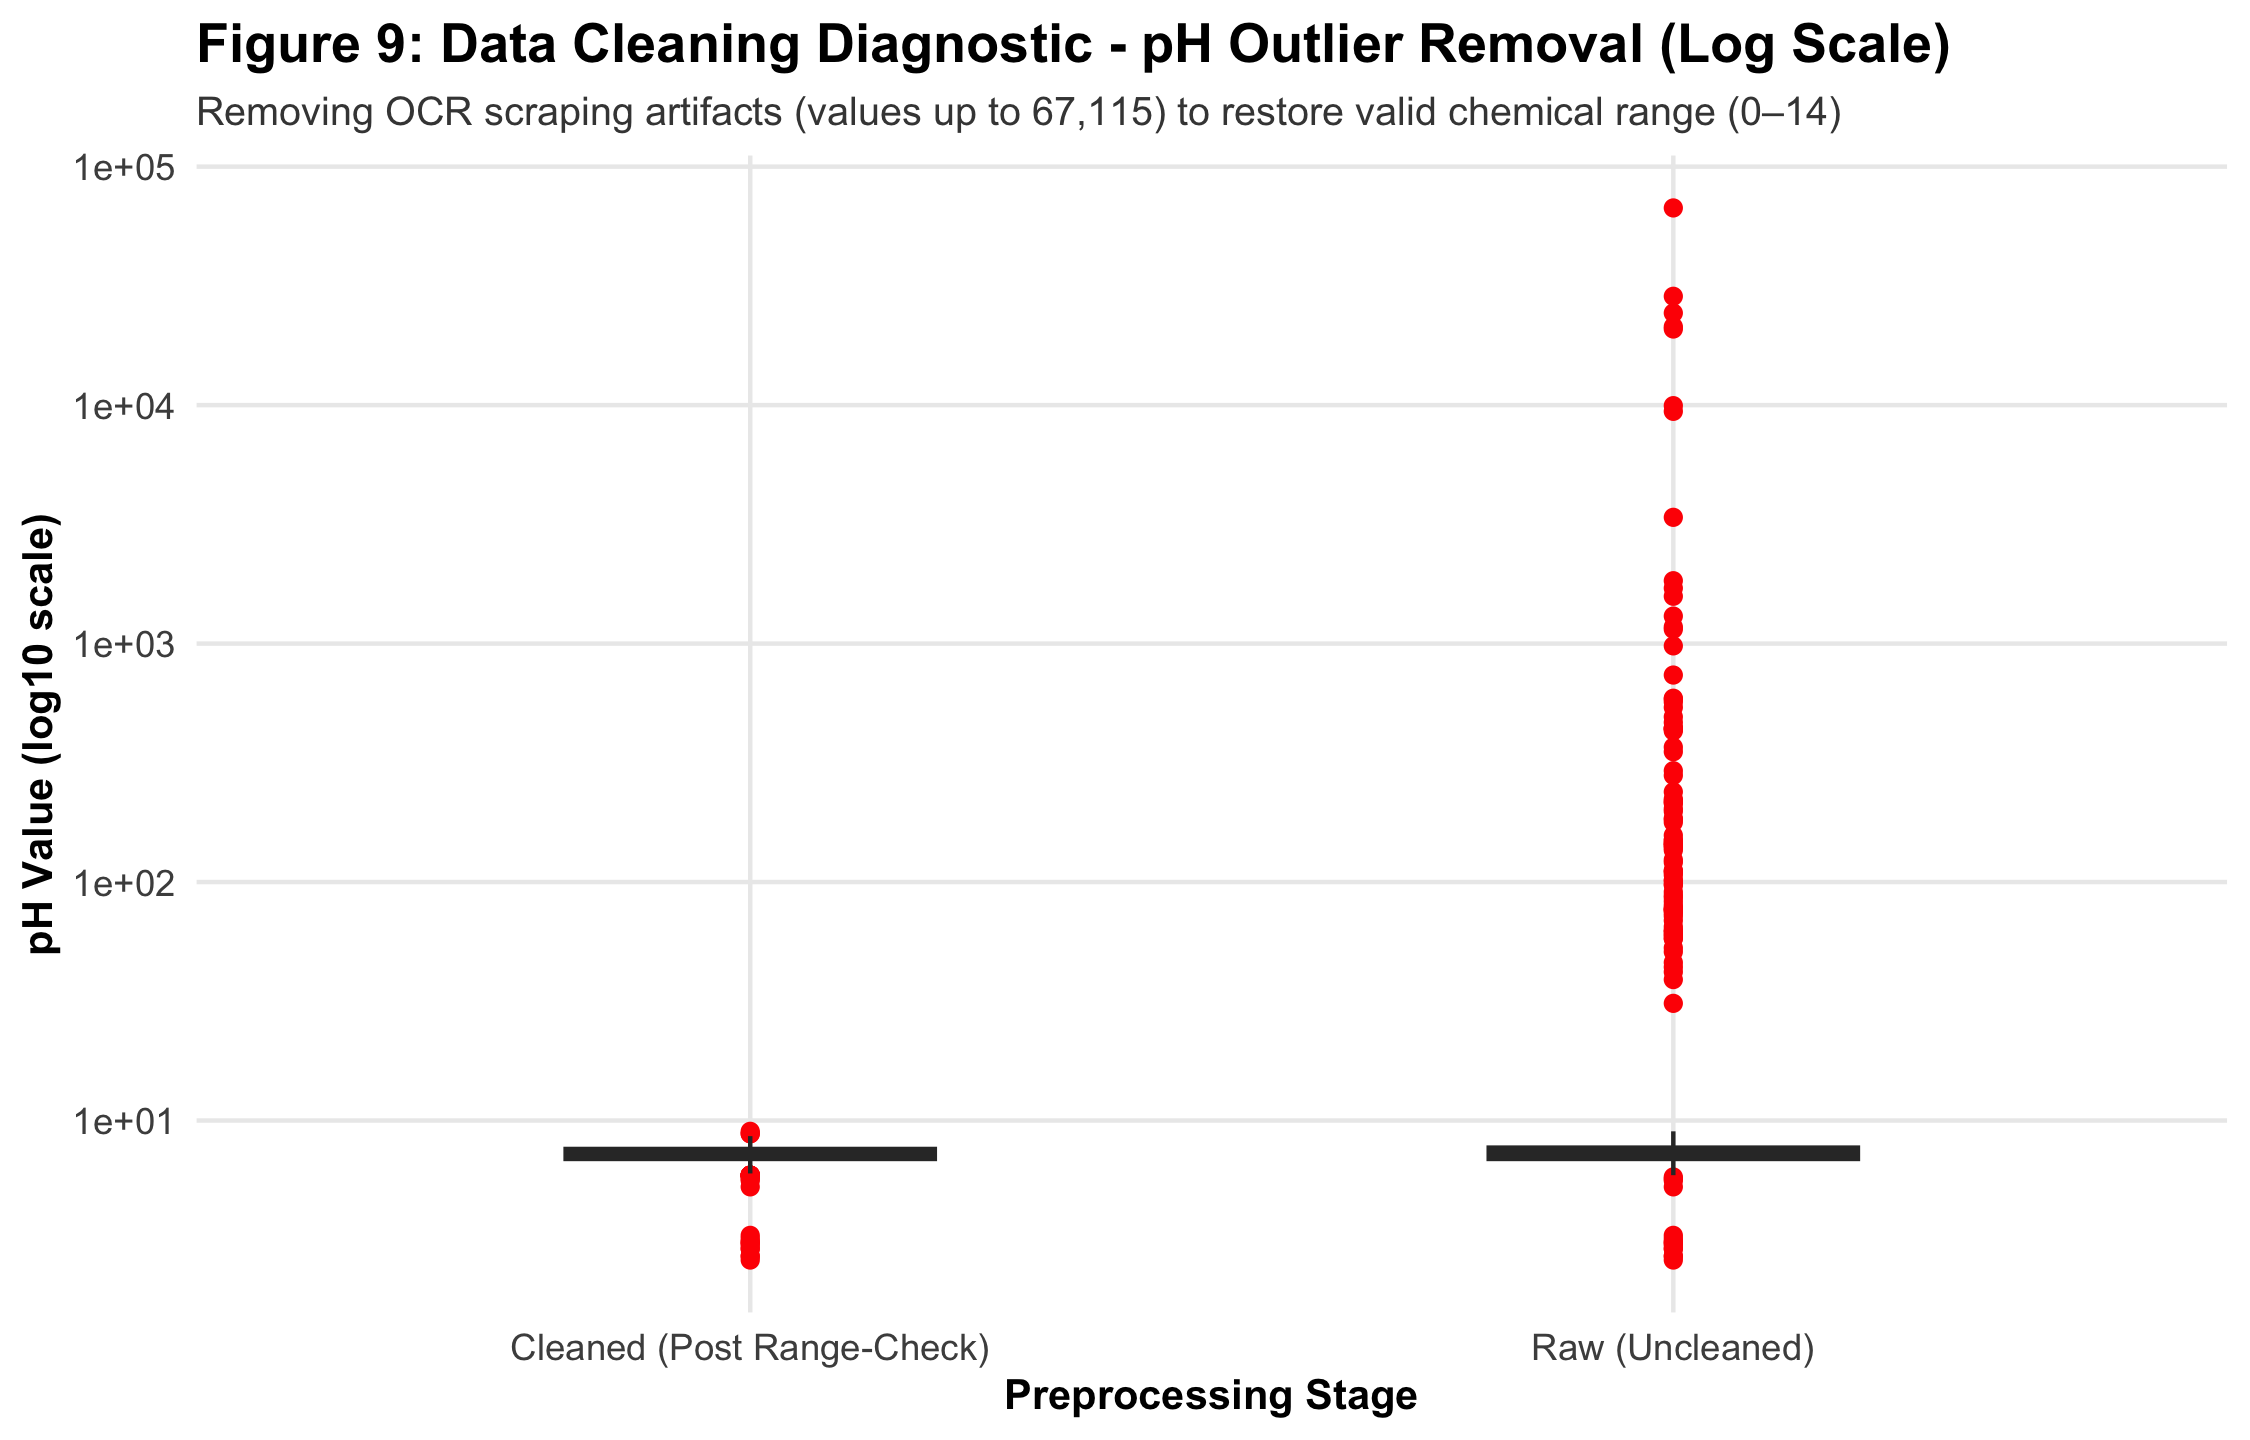
\includegraphics[width=0.85\linewidth]{figures/09_cleaning_before_after_ph} 

}

\caption{Figure: Data Cleaning Diagnostic - Boxplot of Kaggle pH Before and After Outlier Removal (Log Scale)}\label{fig:fig-cleaning-diagnostic}
\end{figure}

\emph{Interpretation of Cleaning Diagnostic:} The raw Kaggle pH
distribution contained extreme outliers (up to \(67,115\)), distorting
the mean and variance. Replacing impossible values with \texttt{NA}
restores the chemically valid range (\(0\) to \(14\)), centering the
median at \(7.30\).

\begin{center}\rule{0.5\linewidth}{0.5pt}\end{center}

\section{Exploratory Data Analysis
(EDA)}\label{exploratory-data-analysis-eda}

\subsection{Univariate Analysis: Core Parameter
Distributions}\label{univariate-analysis-core-parameter-distributions}

We examine the empirical distributions and summary metrics of the four
core water quality parameters from official CPCB monitoring:

\begin{Shaded}
\begin{Highlighting}[]
\NormalTok{core\_summary }\OtherTok{\textless{}{-}}\NormalTok{ df\_cpcb\_master }\SpecialCharTok{\%\textgreater{}\%} 
  \FunctionTok{summarise}\NormalTok{(}\FunctionTok{across}\NormalTok{(}\FunctionTok{c}\NormalTok{(dissolved\_oxygen\_mg\_l, bod\_mg\_l, ph, electrical\_conductivity\_us\_cm), }\FunctionTok{list}\NormalTok{(}
    \AttributeTok{N      =} \SpecialCharTok{\textasciitilde{}}\FunctionTok{sum}\NormalTok{(}\SpecialCharTok{!}\FunctionTok{is.na}\NormalTok{(.)),}
    \AttributeTok{Mean   =} \SpecialCharTok{\textasciitilde{}}\FunctionTok{round}\NormalTok{(}\FunctionTok{mean}\NormalTok{(., }\AttributeTok{na.rm =} \ConstantTok{TRUE}\NormalTok{), }\DecValTok{2}\NormalTok{),}
    \AttributeTok{SD     =} \SpecialCharTok{\textasciitilde{}}\FunctionTok{round}\NormalTok{(}\FunctionTok{sd}\NormalTok{(., }\AttributeTok{na.rm =} \ConstantTok{TRUE}\NormalTok{), }\DecValTok{2}\NormalTok{),}
    \AttributeTok{Median =} \SpecialCharTok{\textasciitilde{}}\FunctionTok{round}\NormalTok{(}\FunctionTok{median}\NormalTok{(., }\AttributeTok{na.rm =} \ConstantTok{TRUE}\NormalTok{), }\DecValTok{2}\NormalTok{),}
    \AttributeTok{IQR    =} \SpecialCharTok{\textasciitilde{}}\FunctionTok{round}\NormalTok{(}\FunctionTok{IQR}\NormalTok{(., }\AttributeTok{na.rm =} \ConstantTok{TRUE}\NormalTok{), }\DecValTok{2}\NormalTok{),}
    \AttributeTok{Min    =} \SpecialCharTok{\textasciitilde{}}\FunctionTok{round}\NormalTok{(}\FunctionTok{min}\NormalTok{(., }\AttributeTok{na.rm =} \ConstantTok{TRUE}\NormalTok{), }\DecValTok{2}\NormalTok{),}
    \AttributeTok{Max    =} \SpecialCharTok{\textasciitilde{}}\FunctionTok{round}\NormalTok{(}\FunctionTok{max}\NormalTok{(., }\AttributeTok{na.rm =} \ConstantTok{TRUE}\NormalTok{), }\DecValTok{2}\NormalTok{)}
\NormalTok{  ), }\AttributeTok{.names =} \StringTok{"\{.col\}\_\_\{.fn\}"}\NormalTok{)) }\SpecialCharTok{\%\textgreater{}\%} 
  \FunctionTok{pivot\_longer}\NormalTok{(}\FunctionTok{everything}\NormalTok{(), }\AttributeTok{names\_to =} \FunctionTok{c}\NormalTok{(}\StringTok{"Parameter"}\NormalTok{, }\StringTok{"Metric"}\NormalTok{), }\AttributeTok{names\_sep =} \StringTok{"\_\_"}\NormalTok{) }\SpecialCharTok{\%\textgreater{}\%} 
  \FunctionTok{pivot\_wider}\NormalTok{(}\AttributeTok{names\_from =}\NormalTok{ Metric, }\AttributeTok{values\_from =}\NormalTok{ value)}

\FunctionTok{kable}\NormalTok{(core\_summary, }\AttributeTok{caption =} \StringTok{"Table 4: Empirical Summary Statistics of Core Water Quality Parameters (CPCB 2018–2021)"}\NormalTok{,}
      \AttributeTok{format.args =} \FunctionTok{list}\NormalTok{(}\AttributeTok{big.mark =} \StringTok{","}\NormalTok{))}
\end{Highlighting}
\end{Shaded}

\begin{longtable}[]{@{}
  >{\raggedright\arraybackslash}p{(\linewidth - 14\tabcolsep) * \real{0.3488}}
  >{\raggedleft\arraybackslash}p{(\linewidth - 14\tabcolsep) * \real{0.0930}}
  >{\raggedleft\arraybackslash}p{(\linewidth - 14\tabcolsep) * \real{0.1047}}
  >{\raggedleft\arraybackslash}p{(\linewidth - 14\tabcolsep) * \real{0.1279}}
  >{\raggedleft\arraybackslash}p{(\linewidth - 14\tabcolsep) * \real{0.0814}}
  >{\raggedleft\arraybackslash}p{(\linewidth - 14\tabcolsep) * \real{0.0698}}
  >{\raggedleft\arraybackslash}p{(\linewidth - 14\tabcolsep) * \real{0.0465}}
  >{\raggedleft\arraybackslash}p{(\linewidth - 14\tabcolsep) * \real{0.1279}}@{}}
\caption{Table 4: Empirical Summary Statistics of Core Water Quality
Parameters (CPCB 2018--2021)}\tabularnewline
\toprule\noalign{}
\begin{minipage}[b]{\linewidth}\raggedright
Parameter
\end{minipage} & \begin{minipage}[b]{\linewidth}\raggedleft
N
\end{minipage} & \begin{minipage}[b]{\linewidth}\raggedleft
Mean
\end{minipage} & \begin{minipage}[b]{\linewidth}\raggedleft
SD
\end{minipage} & \begin{minipage}[b]{\linewidth}\raggedleft
Median
\end{minipage} & \begin{minipage}[b]{\linewidth}\raggedleft
IQR
\end{minipage} & \begin{minipage}[b]{\linewidth}\raggedleft
Min
\end{minipage} & \begin{minipage}[b]{\linewidth}\raggedleft
Max
\end{minipage} \\
\midrule\noalign{}
\endfirsthead
\toprule\noalign{}
\begin{minipage}[b]{\linewidth}\raggedright
Parameter
\end{minipage} & \begin{minipage}[b]{\linewidth}\raggedleft
N
\end{minipage} & \begin{minipage}[b]{\linewidth}\raggedleft
Mean
\end{minipage} & \begin{minipage}[b]{\linewidth}\raggedleft
SD
\end{minipage} & \begin{minipage}[b]{\linewidth}\raggedleft
Median
\end{minipage} & \begin{minipage}[b]{\linewidth}\raggedleft
IQR
\end{minipage} & \begin{minipage}[b]{\linewidth}\raggedleft
Min
\end{minipage} & \begin{minipage}[b]{\linewidth}\raggedleft
Max
\end{minipage} \\
\midrule\noalign{}
\endhead
\bottomrule\noalign{}
\endlastfoot
dissolved\_oxygen\_mg\_l & 96,978 & 6.54 & 1.87 & 6.80 & 1.9 & 0 & 25 \\
bod\_mg\_l & 84,272 & 5.76 & 16.26 & 2.30 & 2.4 & 0 & 1,315 \\
ph & 107,342 & 7.53 & 0.61 & 7.58 & 0.7 & 2 & 14 \\
electrical\_conductivity\_us\_cm & 48,160 & 3,474.51 & 171,820.62 &
395.00 & 749.0 & 1 & 25,392,600 \\
\end{longtable}

\begin{Shaded}
\begin{Highlighting}[]
\NormalTok{knitr}\SpecialCharTok{::}\FunctionTok{include\_graphics}\NormalTok{(}\FunctionTok{file.path}\NormalTok{(FIG\_DIR, }\StringTok{"03\_water\_quality\_distributions.png"}\NormalTok{))}
\end{Highlighting}
\end{Shaded}

\begin{figure}

{\centering 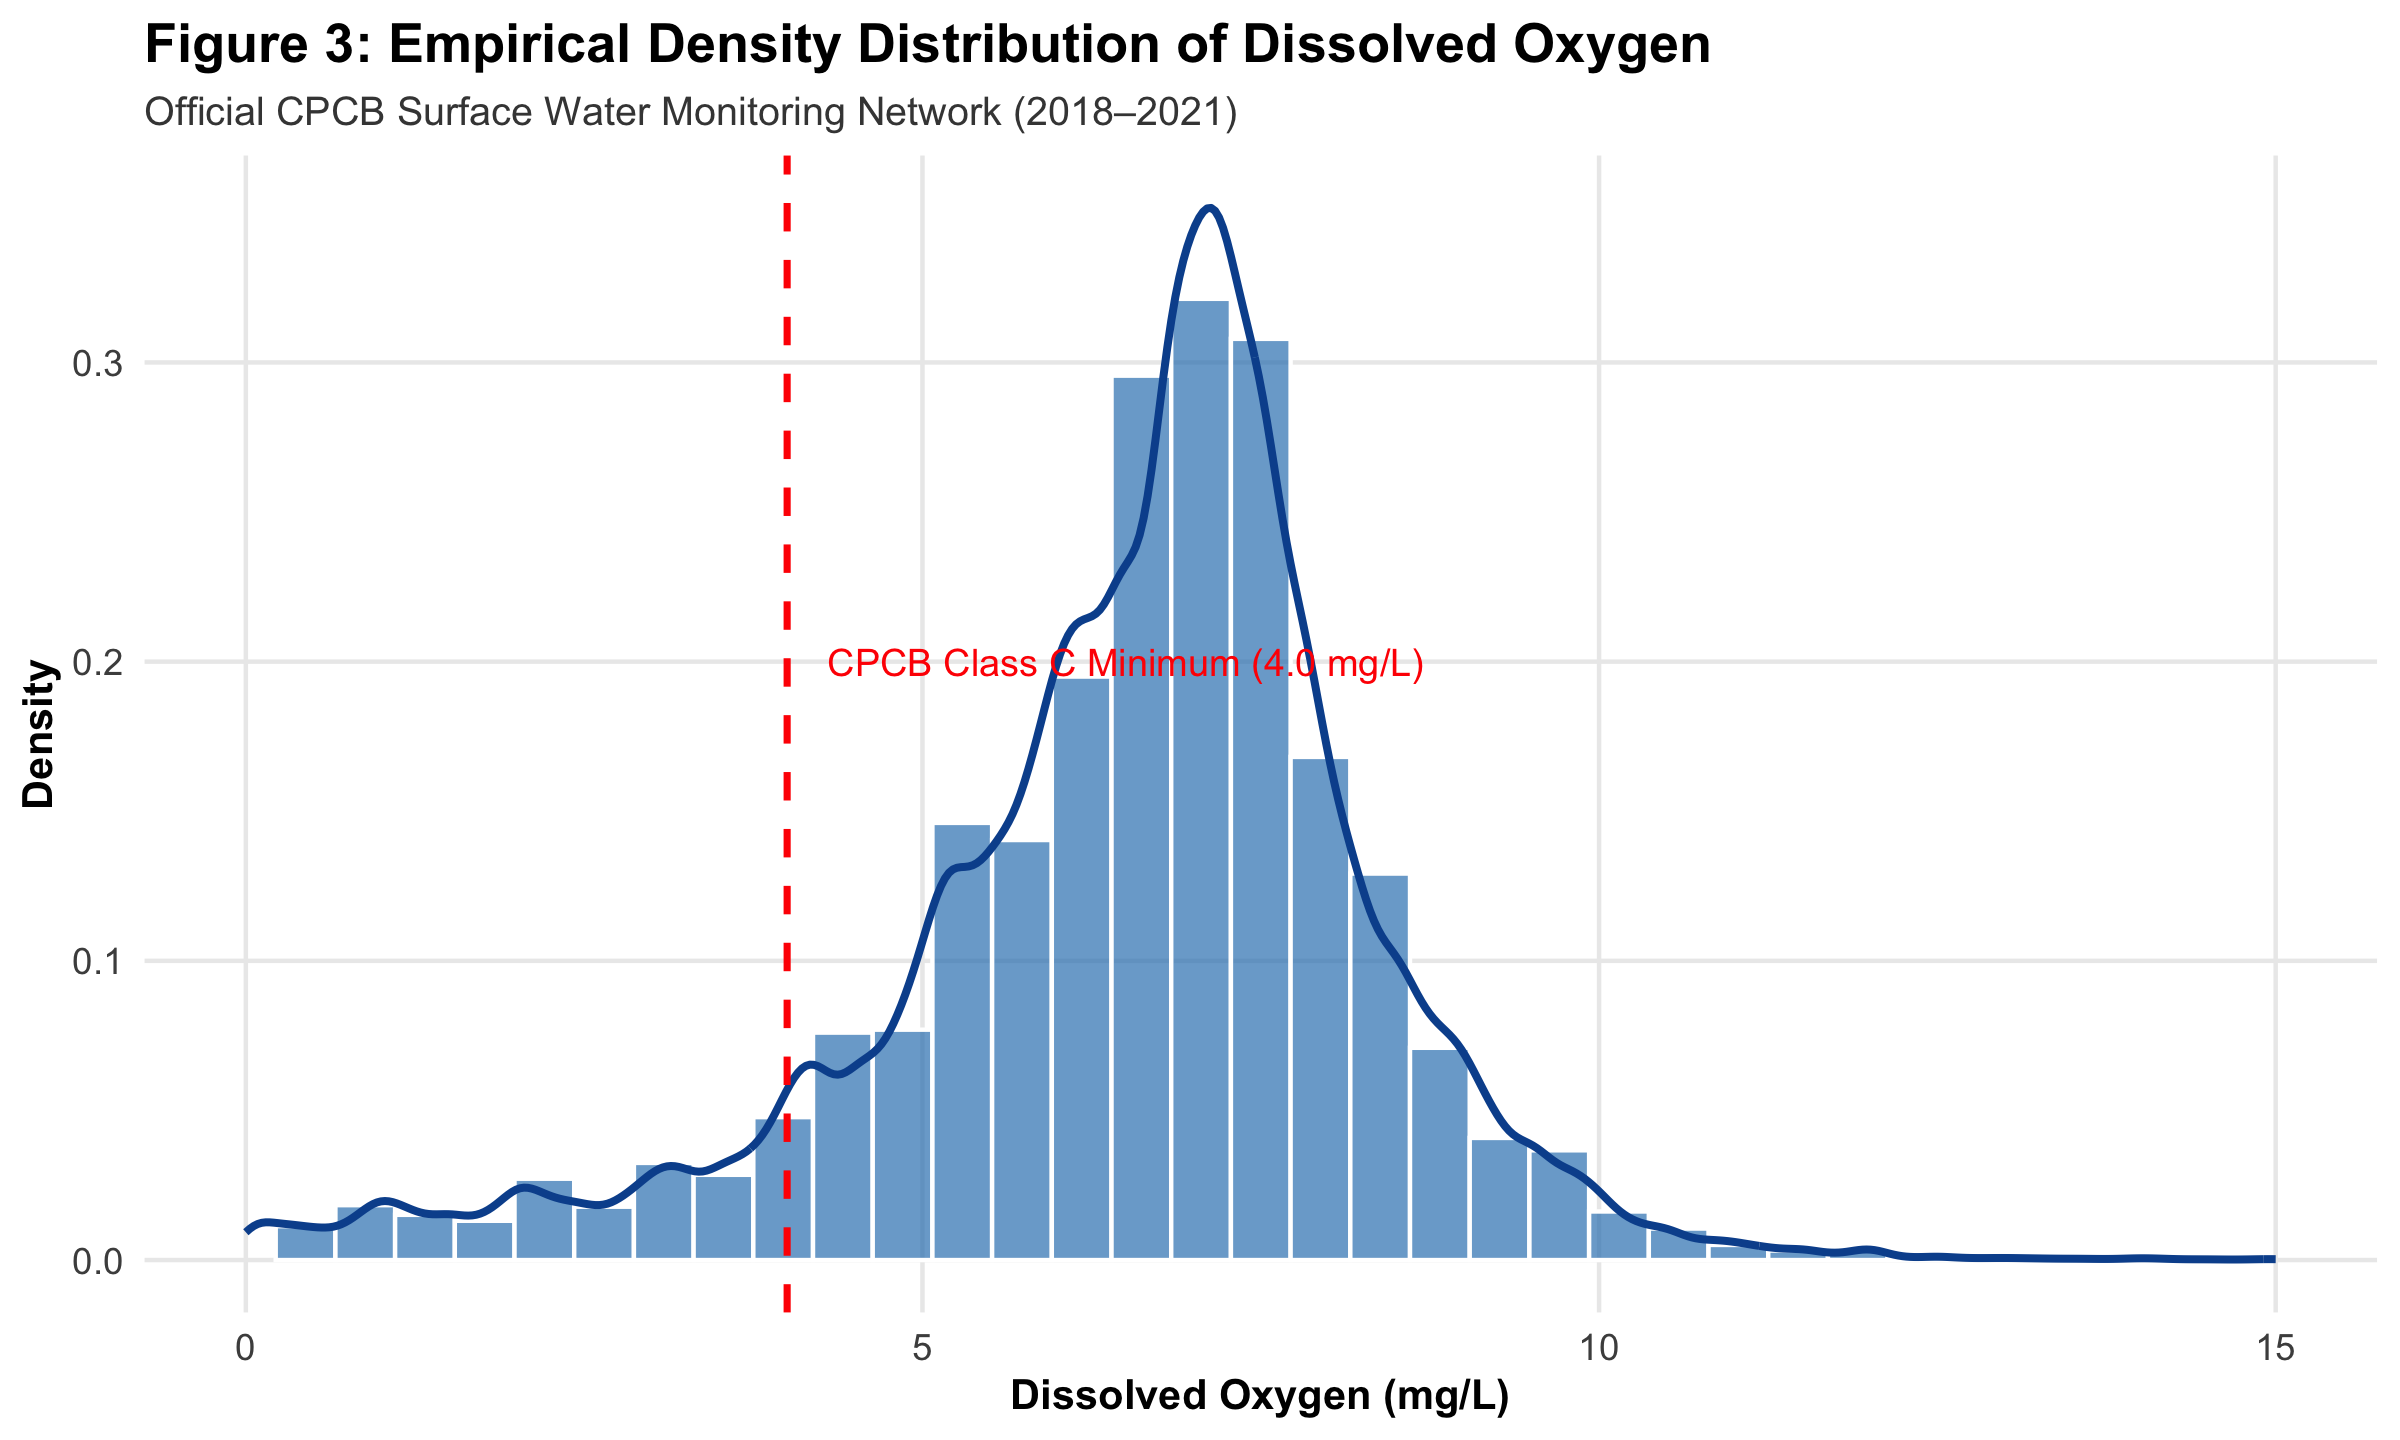
\includegraphics[width=0.85\linewidth]{figures/03_water_quality_distributions} 

}

\caption{Figure: Empirical Density Distribution of Dissolved Oxygen (CPCB 2018–2021)}\label{fig:fig-do-dist}
\end{figure}

\emph{Interpretation of DO Distribution:} Dissolved Oxygen exhibits a
unimodal, slightly left-skewed distribution centered at a median of
\(6.80\text{ mg/L}\) (\(Mean = 6.54\text{ mg/L}\)). Approximately
\(9.2\%\) of observations fall below the CPCB Class C standard of
\(4.0\text{ mg/L}\), indicating localized hypoxic conditions in polluted
stretches.

\subsection{Geographic Variation}\label{geographic-variation}

\begin{Shaded}
\begin{Highlighting}[]
\NormalTok{knitr}\SpecialCharTok{::}\FunctionTok{include\_graphics}\NormalTok{(}\FunctionTok{file.path}\NormalTok{(FIG\_DIR, }\StringTok{"02\_cpcb\_geographic\_stations\_map.png"}\NormalTok{))}
\end{Highlighting}
\end{Shaded}

\begin{figure}

{\centering 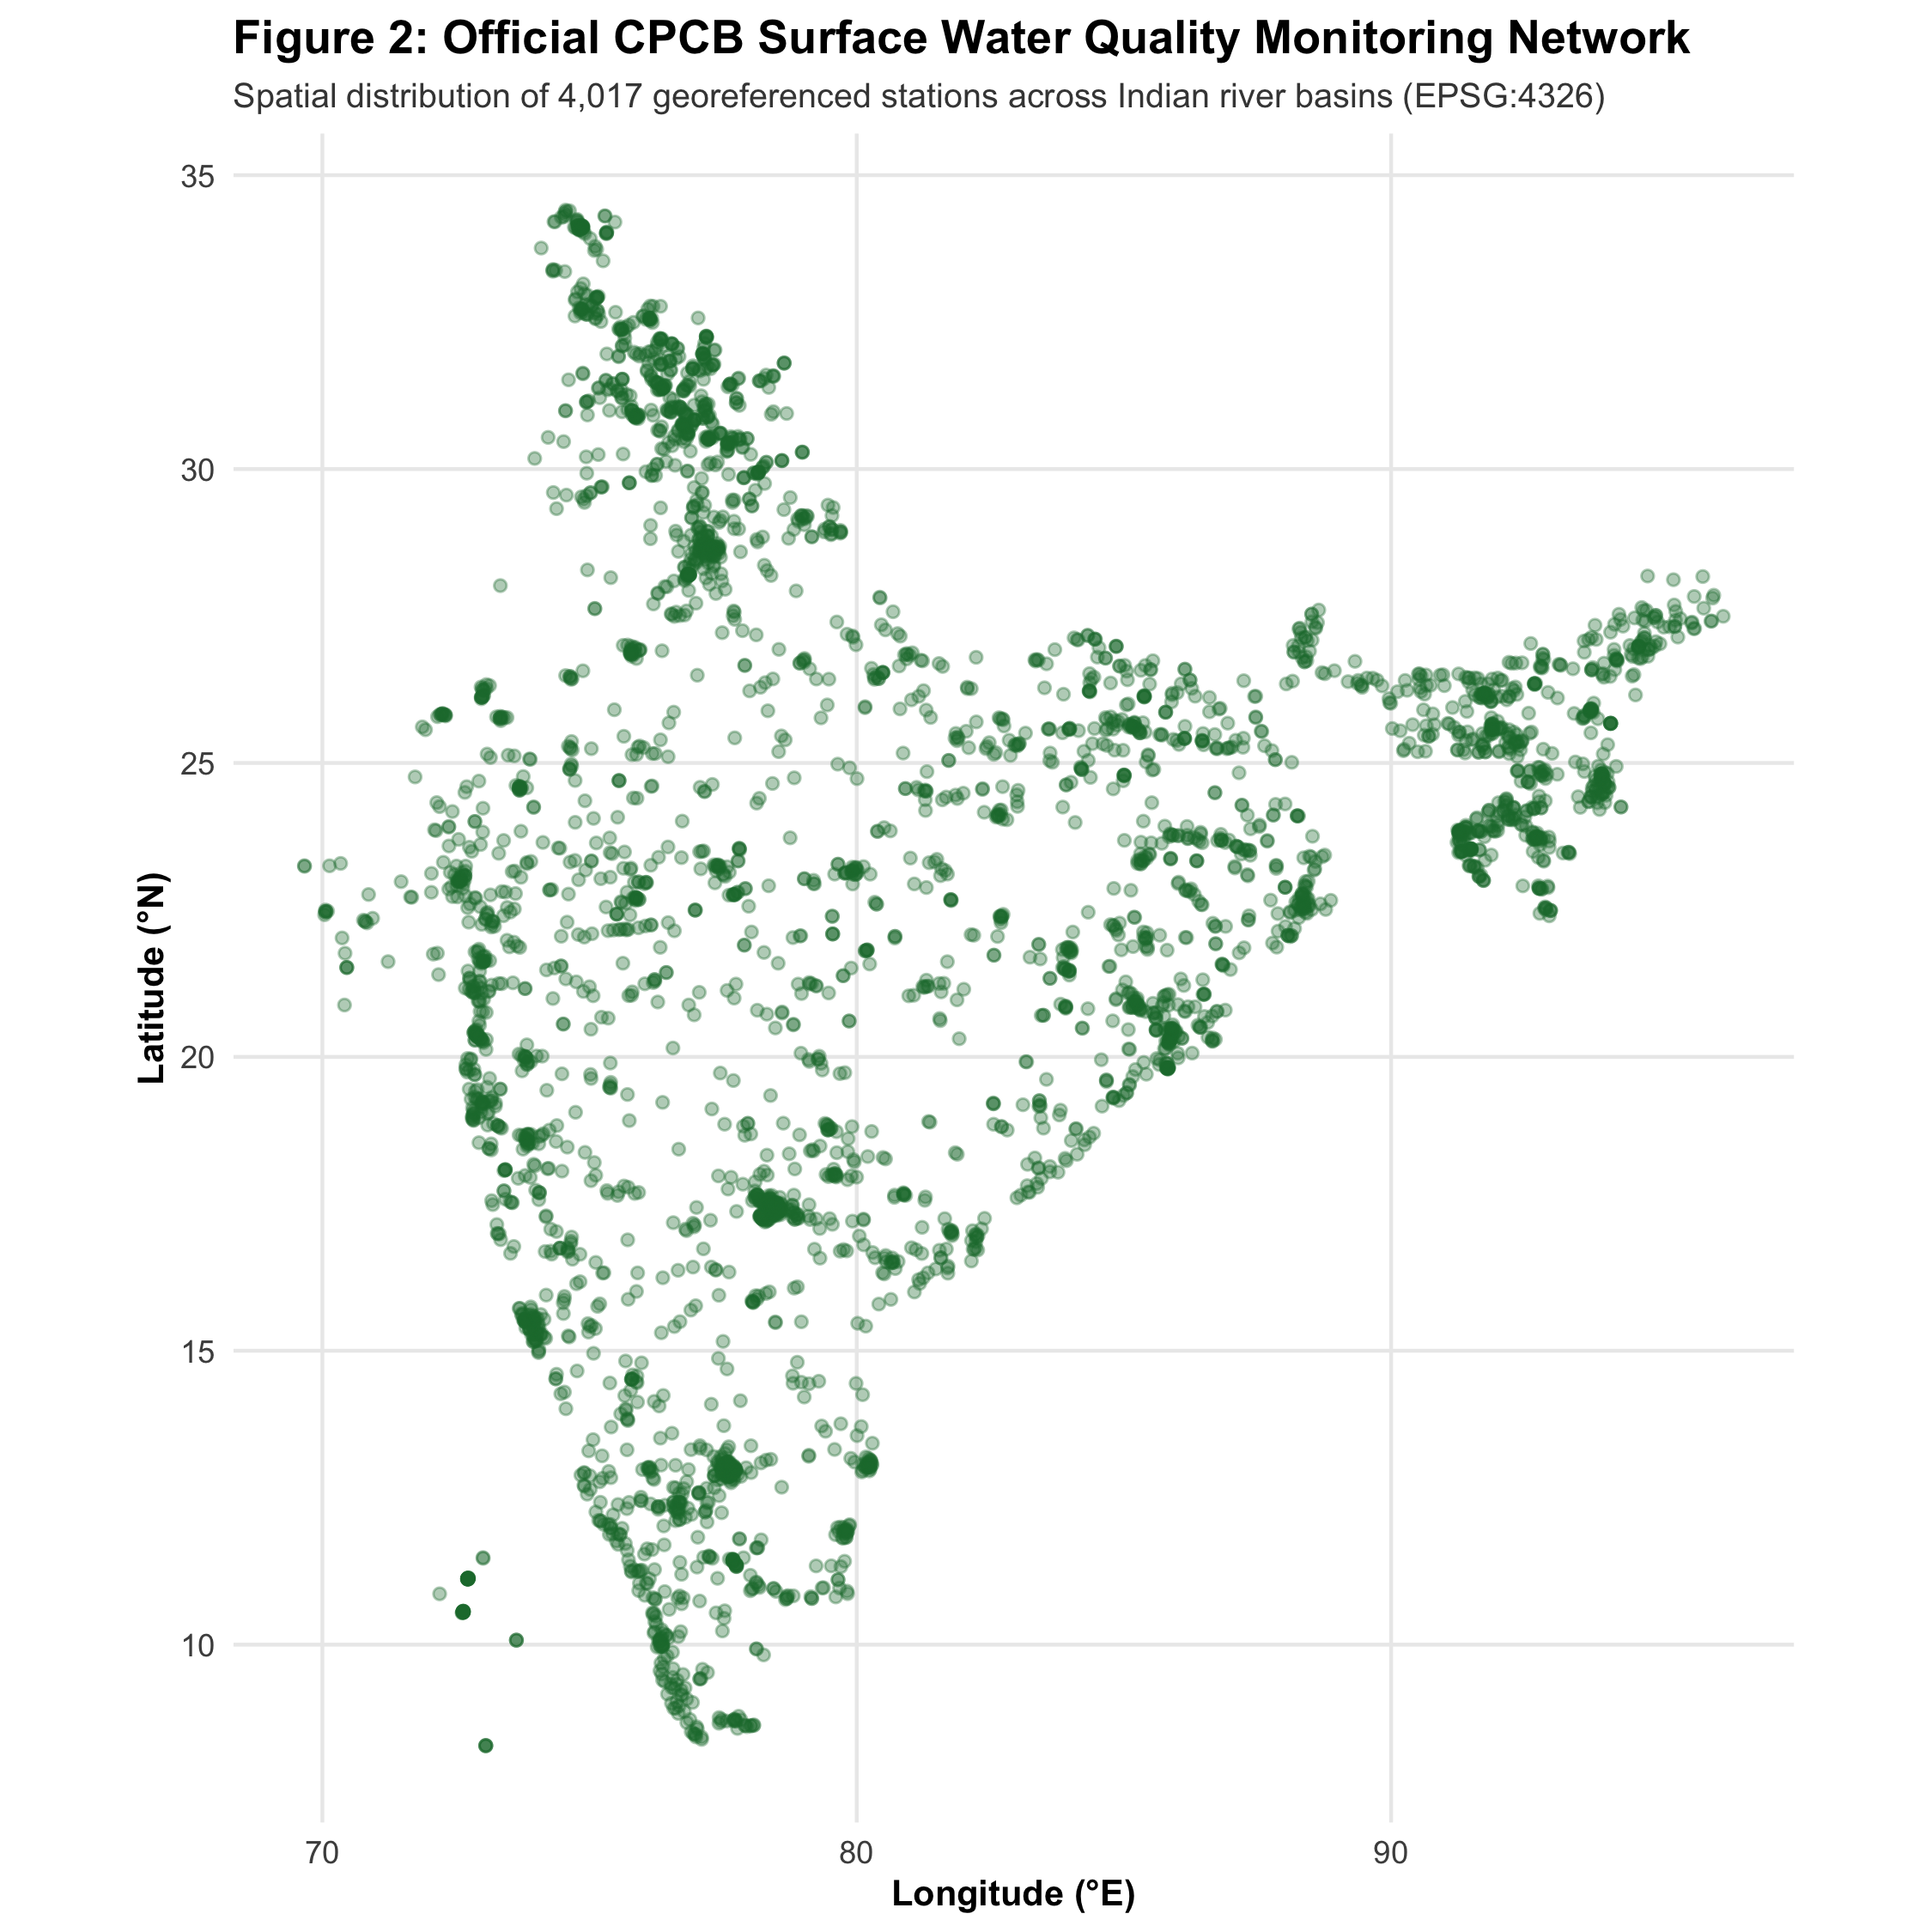
\includegraphics[width=0.8\linewidth]{figures/02_cpcb_geographic_stations_map} 

}

\caption{Figure: Official CPCB Monitoring Stations Across India (WGS84 Coordinates)}\label{fig:fig-stations-map}
\end{figure}

\emph{Interpretation of Spatial Map:} The CPCB monitoring network spans
4,017 stations across all major river basins, including the Indus,
Ganga, Brahmaputra, Godavari, Krishna, Mahanadi, and Cauvery. Dense
station clustering appears in industrialized and densely populated
corridors in Maharashtra, Gujarat, Uttar Pradesh, and Tamil Nadu.

\begin{Shaded}
\begin{Highlighting}[]
\NormalTok{knitr}\SpecialCharTok{::}\FunctionTok{include\_graphics}\NormalTok{(}\FunctionTok{file.path}\NormalTok{(FIG\_DIR, }\StringTok{"10\_state\_observation\_counts.png"}\NormalTok{))}
\end{Highlighting}
\end{Shaded}

\begin{figure}

{\centering 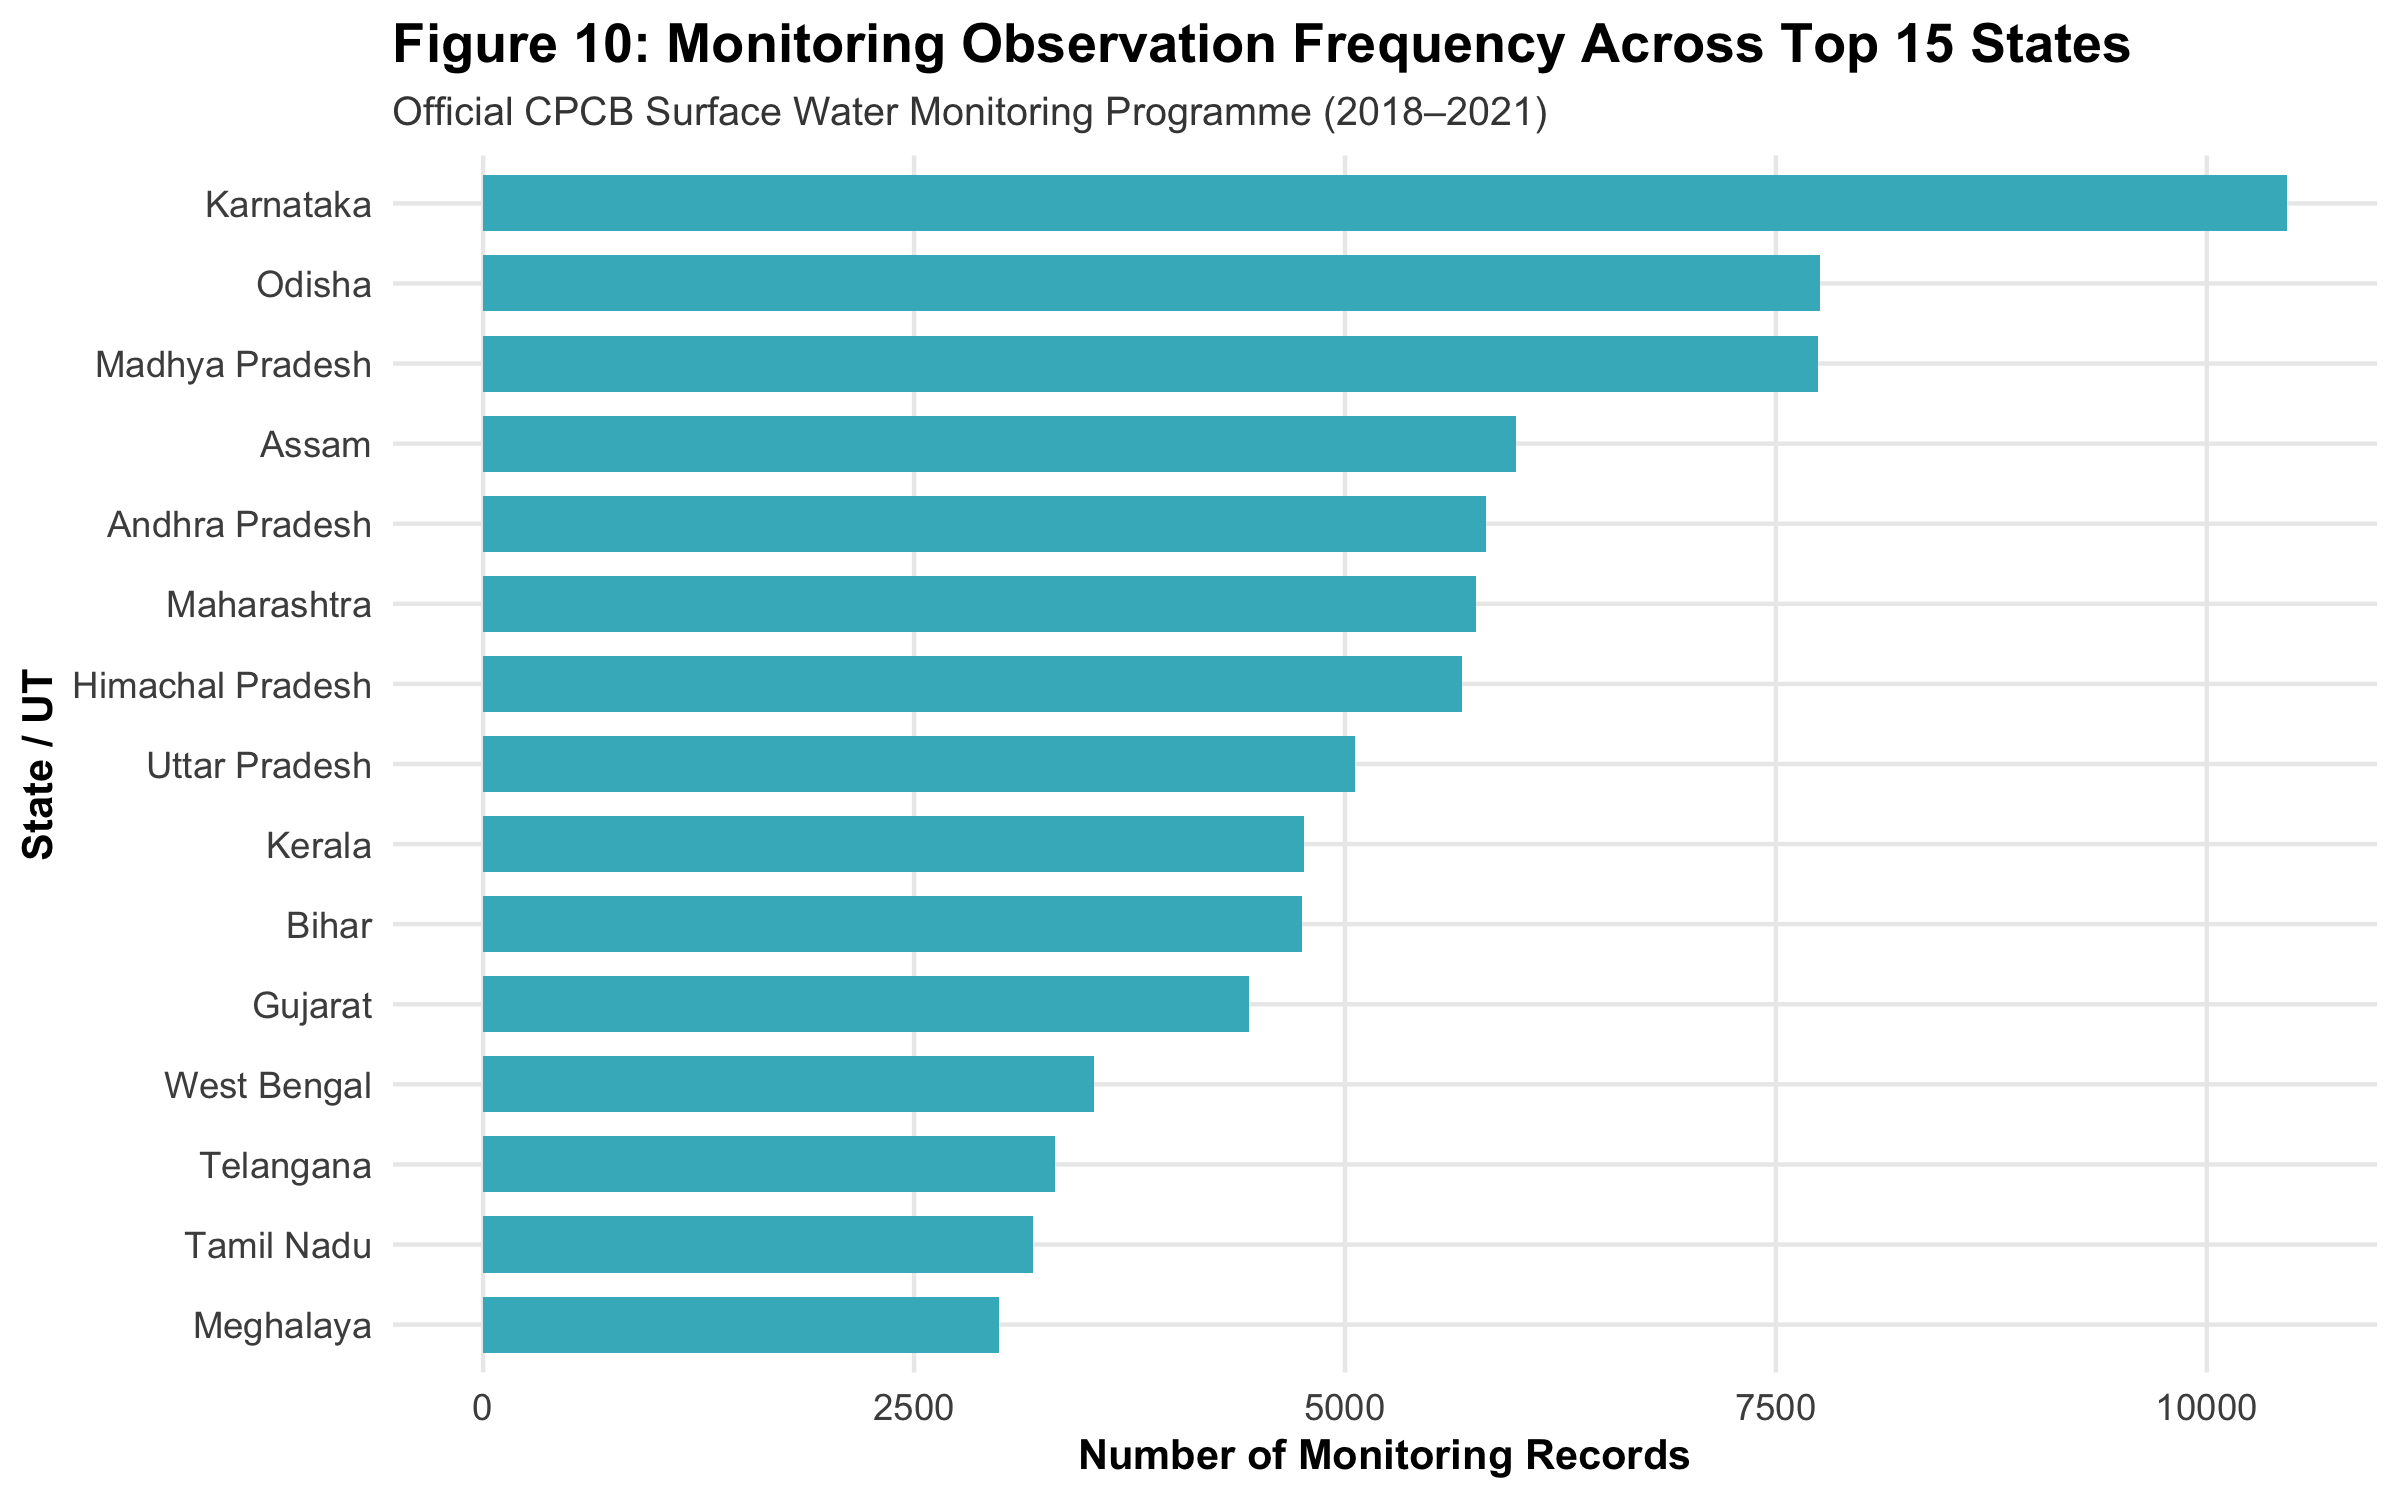
\includegraphics[width=0.85\linewidth]{figures/10_state_observation_counts} 

}

\caption{Figure: Monitoring Observation Frequency Across Top 15 Indian States}\label{fig:fig-state-counts}
\end{figure}

\begin{Shaded}
\begin{Highlighting}[]
\NormalTok{knitr}\SpecialCharTok{::}\FunctionTok{include\_graphics}\NormalTok{(}\FunctionTok{file.path}\NormalTok{(FIG\_DIR, }\StringTok{"04\_state\_dissolved\_oxygen\_boxplot.png"}\NormalTok{))}
\end{Highlighting}
\end{Shaded}

\begin{figure}

{\centering 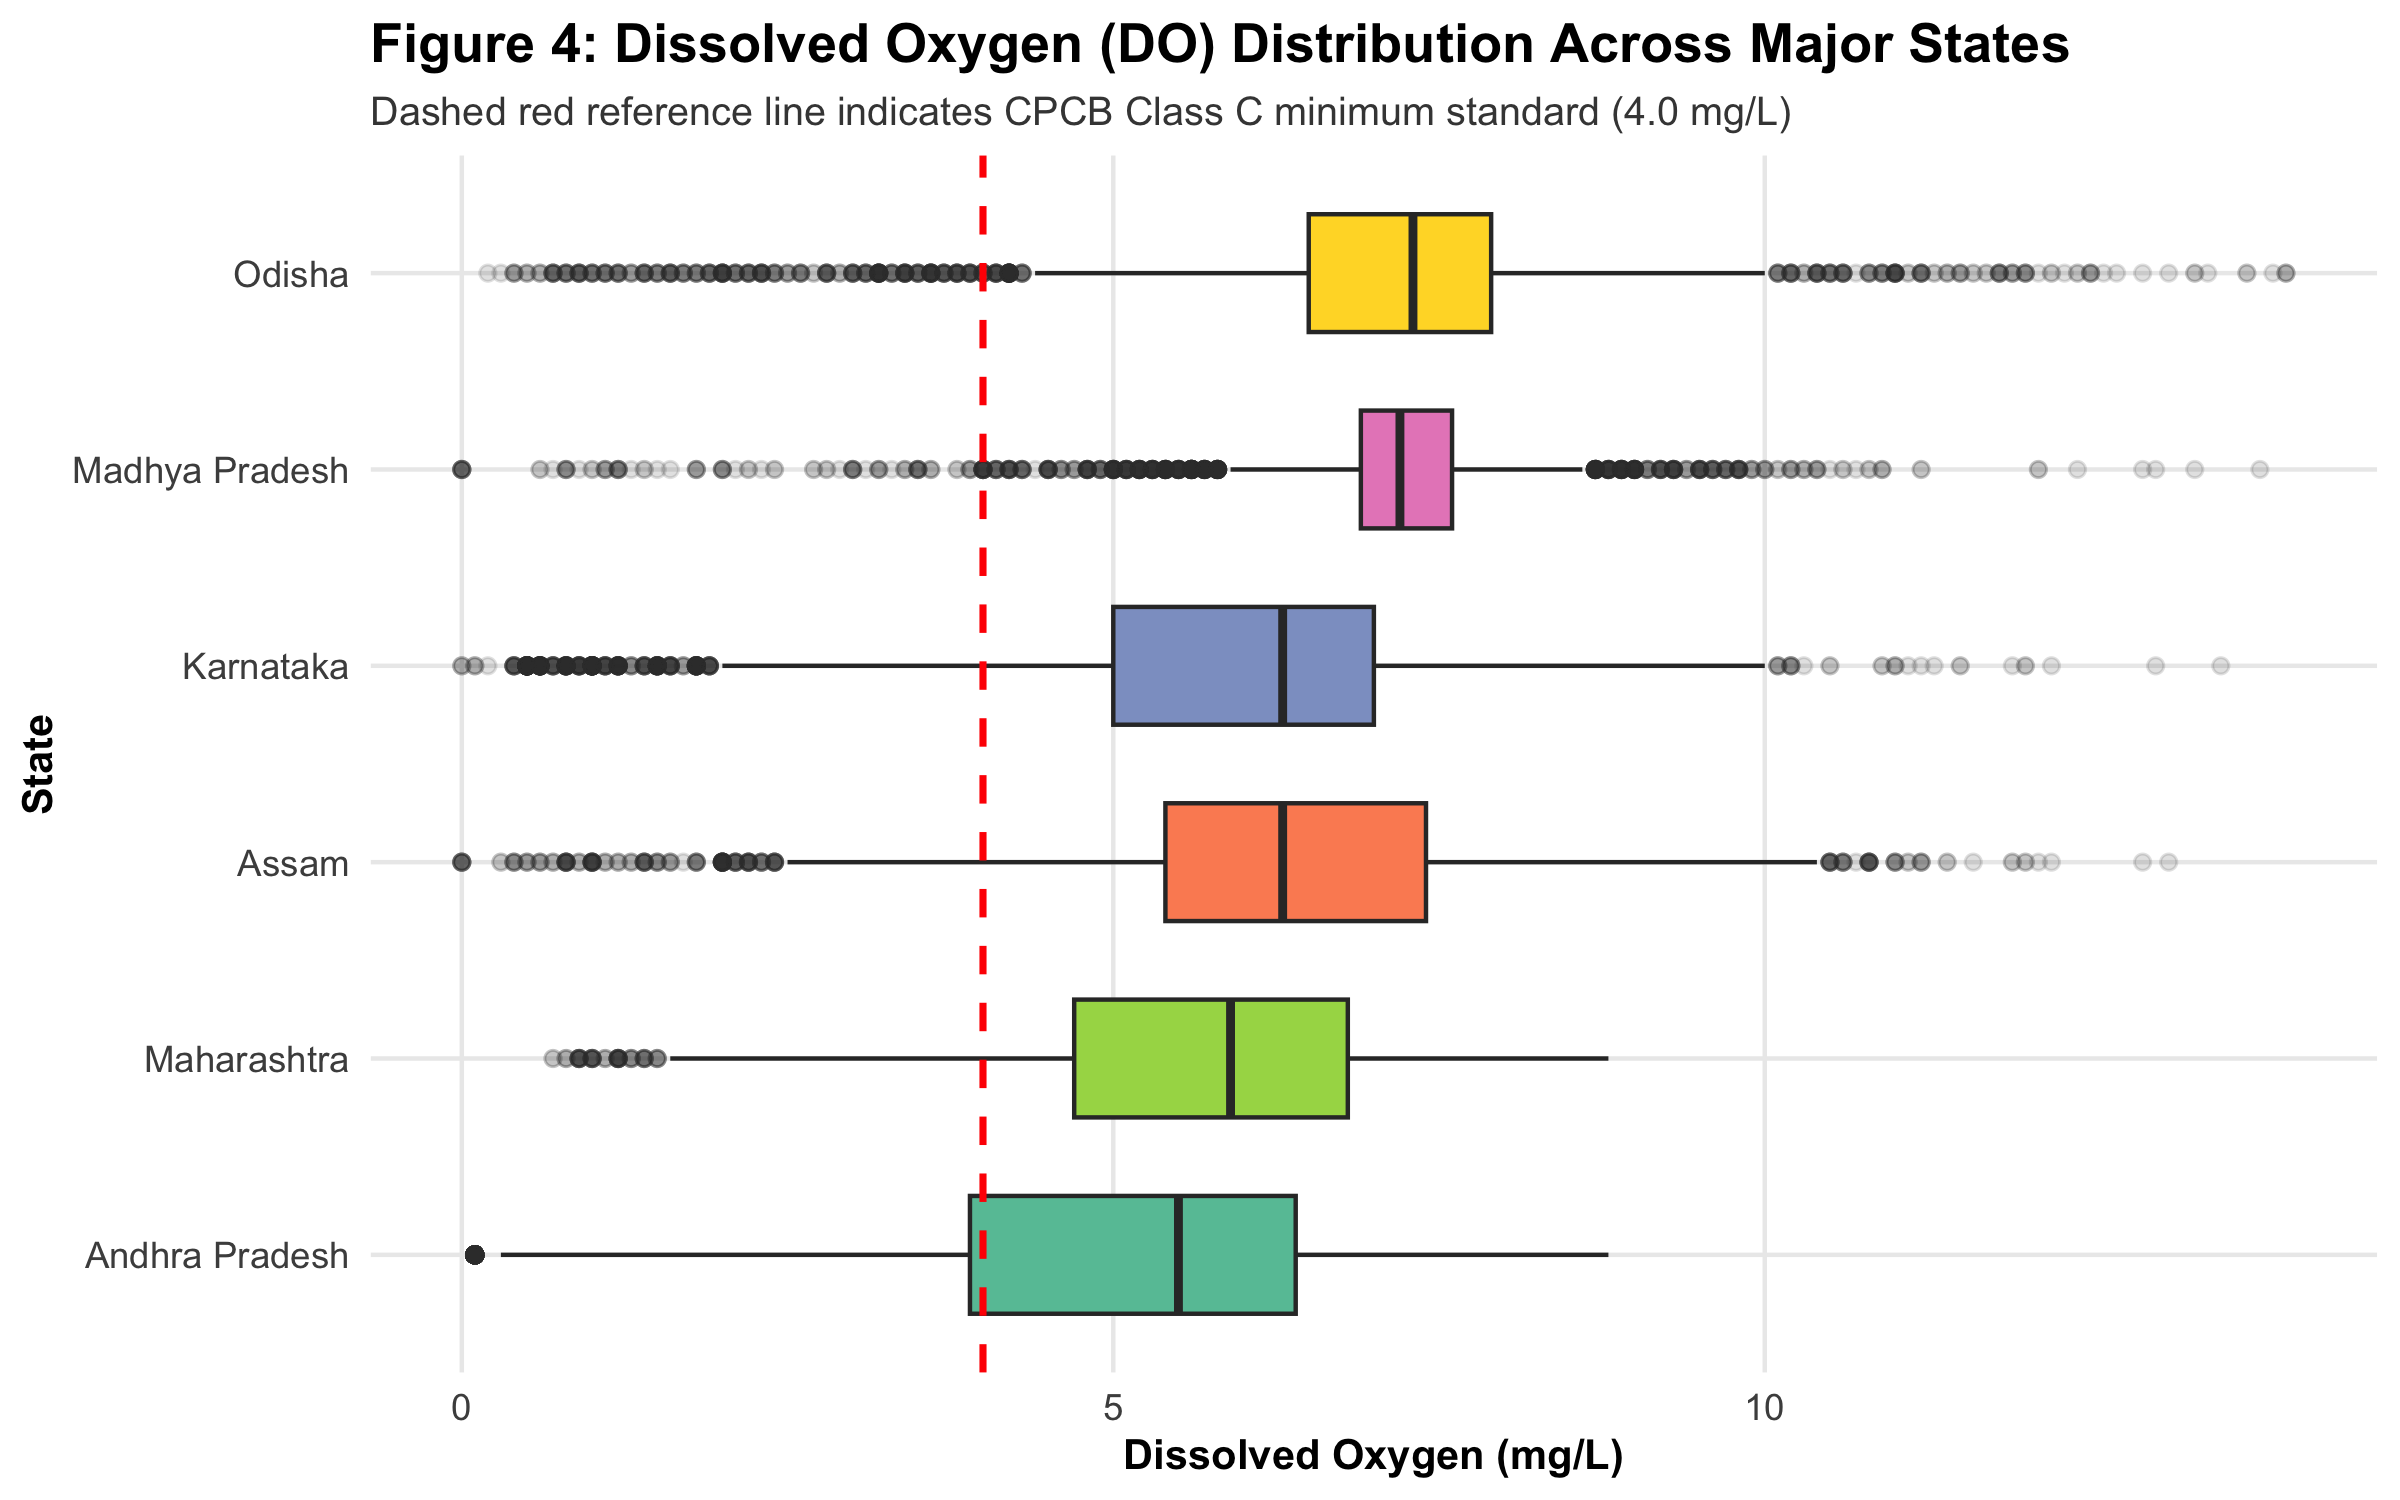
\includegraphics[width=0.85\linewidth]{figures/04_state_dissolved_oxygen_boxplot} 

}

\caption{Figure: State-wise Distribution of Dissolved Oxygen Across Major States}\label{fig:fig-state-do-boxplot}
\end{figure}

\emph{Interpretation of State-wise DO Comparison:} Himalayan and
southern coastal states (such as Himachal Pradesh, Kerala, and Goa)
maintain consistently high median DO levels (\(> 7.5\text{ mg/L}\)).
Conversely, states with intensive urban and industrial discharge exhibit
wider interquartile ranges and frequent sub-\(4.0\text{ mg/L}\)
outliers.

We test whether regional variations in BOD are statistically significant
across the top monitoring states using the non-parametric
\textbf{Kruskal-Wallis Rank-Sum Test}:

\begin{Shaded}
\begin{Highlighting}[]
\NormalTok{top\_states }\OtherTok{\textless{}{-}}\NormalTok{ df\_cpcb\_master }\SpecialCharTok{\%\textgreater{}\%} 
  \FunctionTok{count}\NormalTok{(state, }\AttributeTok{sort =} \ConstantTok{TRUE}\NormalTok{) }\SpecialCharTok{\%\textgreater{}\%} 
  \FunctionTok{filter}\NormalTok{(}\SpecialCharTok{!}\FunctionTok{is.na}\NormalTok{(state)) }\SpecialCharTok{\%\textgreater{}\%} 
  \FunctionTok{slice\_head}\NormalTok{(}\AttributeTok{n =} \DecValTok{6}\NormalTok{) }\SpecialCharTok{\%\textgreater{}\%} 
  \FunctionTok{pull}\NormalTok{(state)}

\NormalTok{kw\_test }\OtherTok{\textless{}{-}} \FunctionTok{kruskal.test}\NormalTok{(bod\_mg\_l }\SpecialCharTok{\textasciitilde{}}\NormalTok{ state, }\AttributeTok{data =}\NormalTok{ df\_cpcb\_master }\SpecialCharTok{\%\textgreater{}\%} \FunctionTok{filter}\NormalTok{(state }\SpecialCharTok{\%in\%}\NormalTok{ top\_states))}
\NormalTok{kw\_test}
\end{Highlighting}
\end{Shaded}

\begin{verbatim}
## 
##  Kruskal-Wallis rank sum test
## 
## data:  bod_mg_l by state
## Kruskal-Wallis chi-squared = 11726, df = 5, p-value < 2.2e-16
\end{verbatim}

The test reveals statistically significant differences in organic
pollution load across states
(\(\chi^2 = \ensuremath{1.172565\times 10^{4}}\),
\(p < 2.2 \times 10^{-16}\)).

\subsection{Seasonal Dynamics and Monsoon
Dilution}\label{seasonal-dynamics-and-monsoon-dilution}

Seasonal variation affects both chemical reaction kinetics and
volumetric dilution:

\begin{Shaded}
\begin{Highlighting}[]
\NormalTok{knitr}\SpecialCharTok{::}\FunctionTok{include\_graphics}\NormalTok{(}\FunctionTok{file.path}\NormalTok{(FIG\_DIR, }\StringTok{"05\_seasonal\_bod\_variation.png"}\NormalTok{))}
\end{Highlighting}
\end{Shaded}

\begin{figure}

{\centering 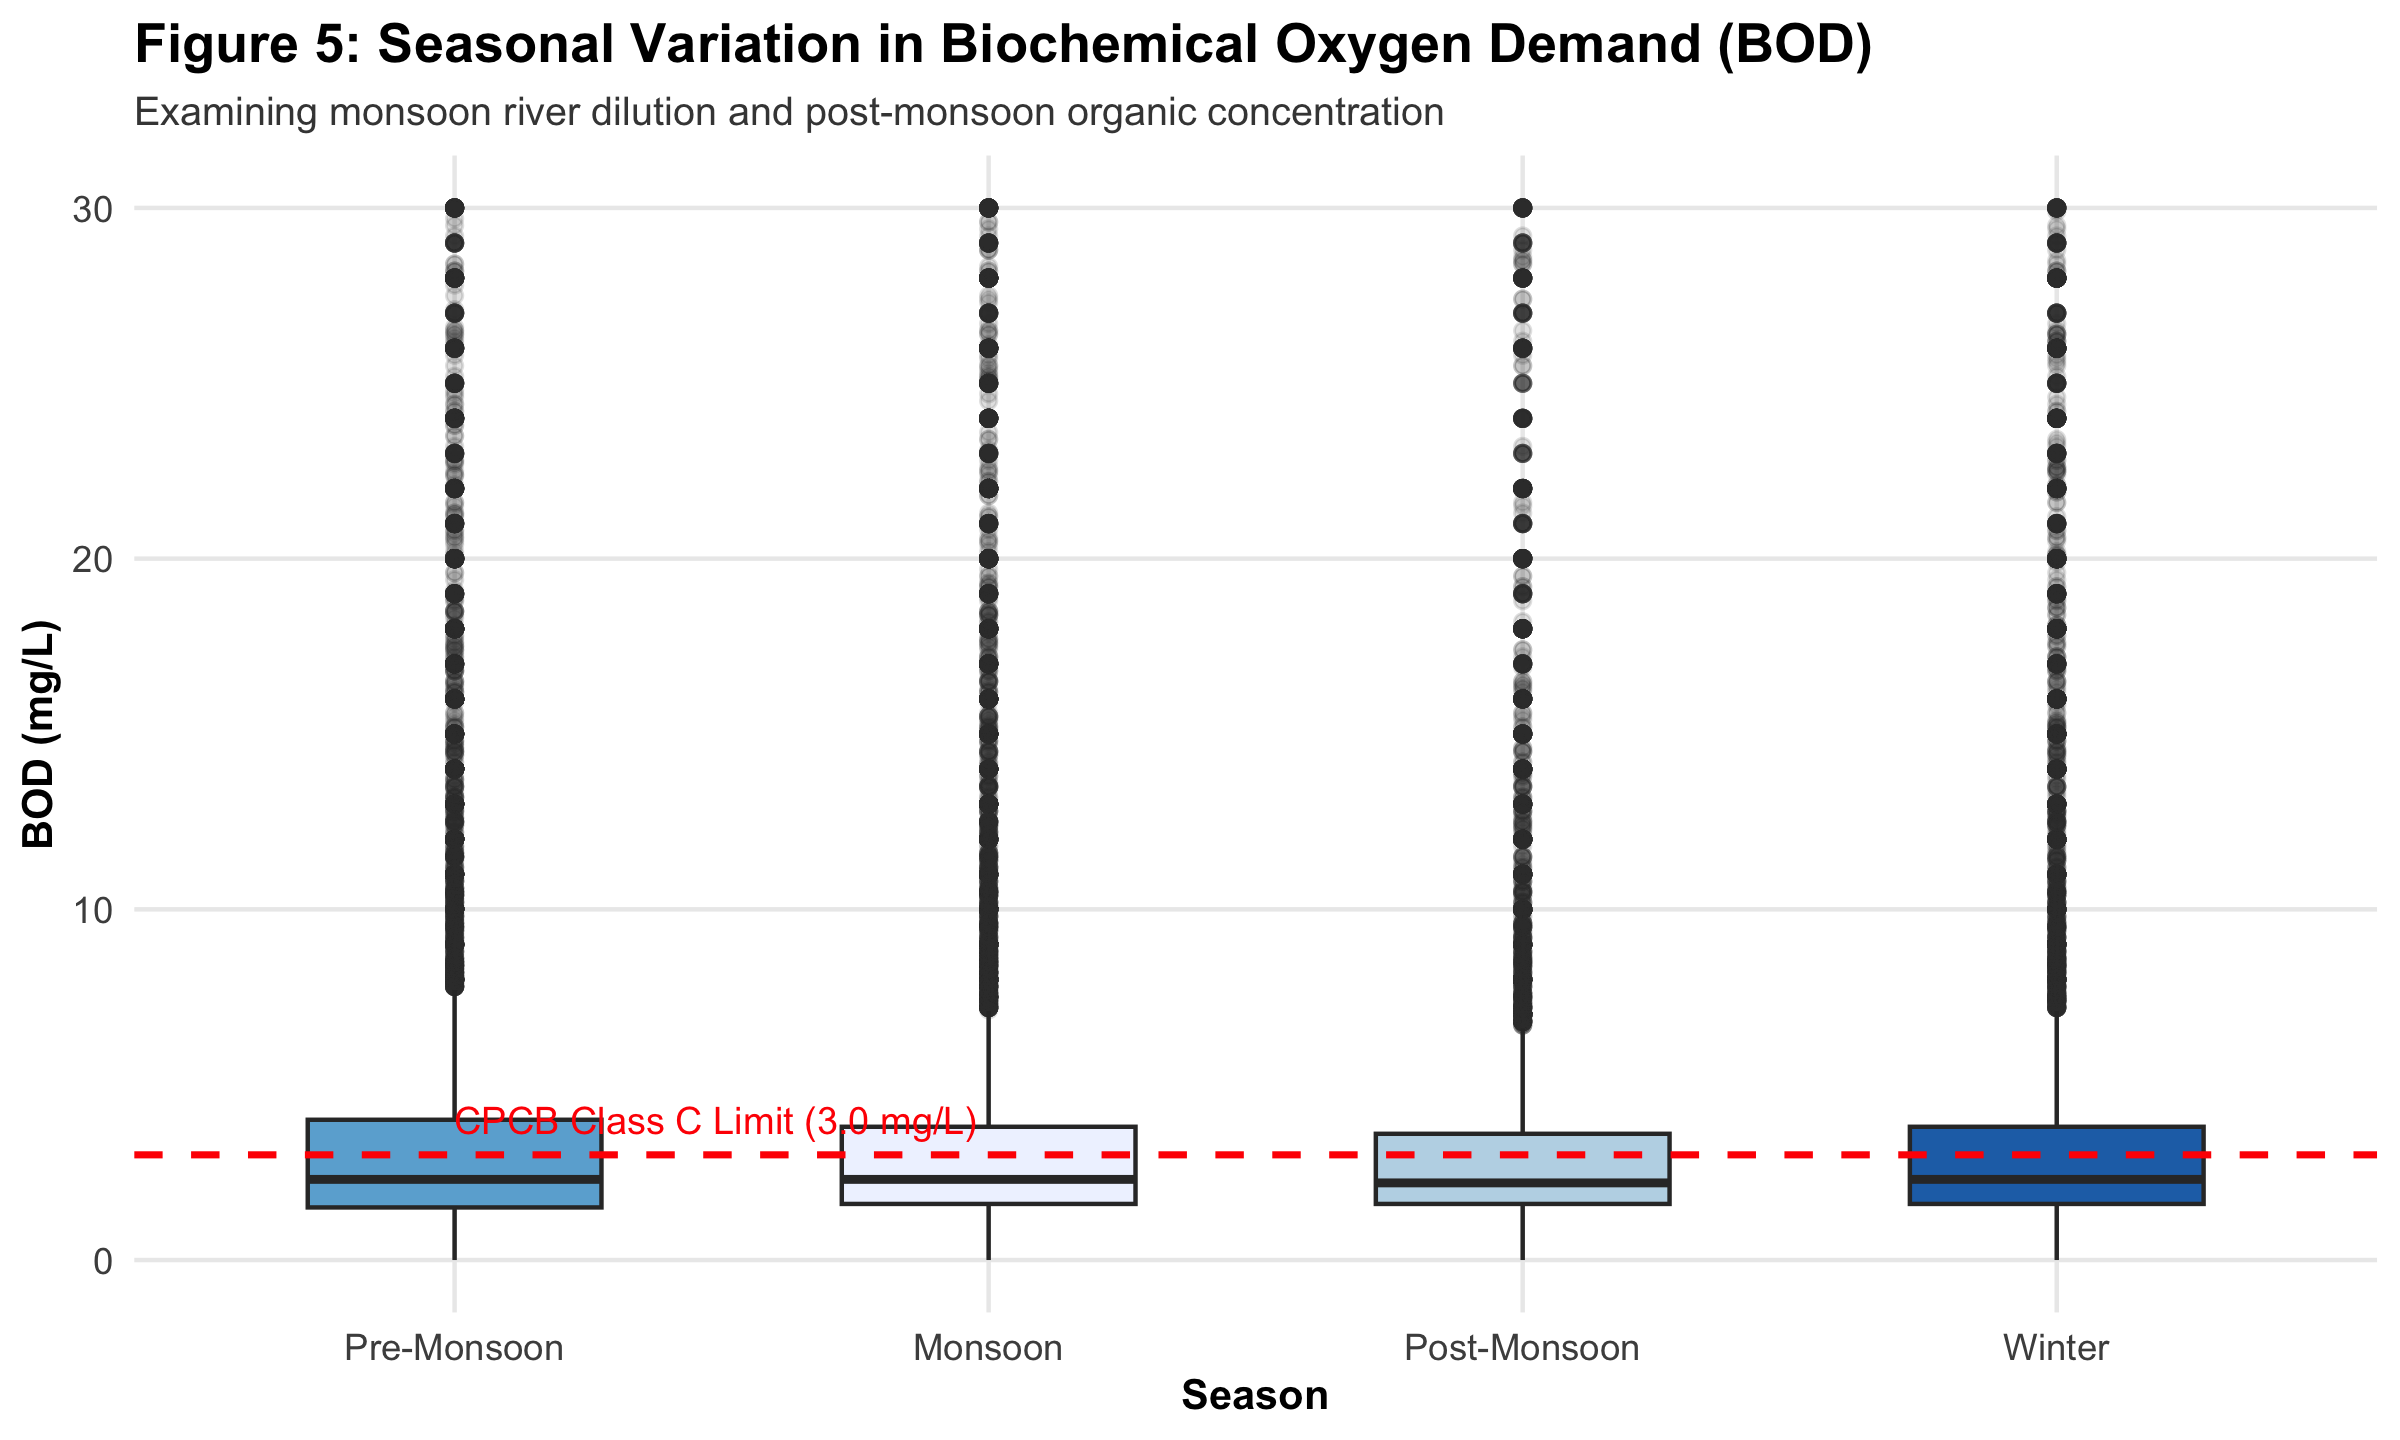
\includegraphics[width=0.85\linewidth]{figures/05_seasonal_bod_variation} 

}

\caption{Figure: Seasonal Variation in Biochemical Oxygen Demand (BOD)}\label{fig:fig-seasonal-bod}
\end{figure}

\emph{Interpretation of Seasonal BOD Boxplot:} During the monsoon season
(June--September), median BOD drops to \(2.10\text{ mg/L}\) compared to
\(2.40\text{ mg/L}\) in the pre-monsoon summer, demonstrating the
diluting effect of high river discharge.

We formally evaluate the seasonal shift in Dissolved Oxygen between
Pre-Monsoon and Monsoon periods using the \textbf{Wilcoxon Rank-Sum
Test}:

\begin{Shaded}
\begin{Highlighting}[]
\NormalTok{season\_sub }\OtherTok{\textless{}{-}}\NormalTok{ df\_cpcb\_master }\SpecialCharTok{\%\textgreater{}\%} 
  \FunctionTok{filter}\NormalTok{(season }\SpecialCharTok{\%in\%} \FunctionTok{c}\NormalTok{(}\StringTok{"Pre{-}Monsoon"}\NormalTok{, }\StringTok{"Monsoon"}\NormalTok{), }\SpecialCharTok{!}\FunctionTok{is.na}\NormalTok{(dissolved\_oxygen\_mg\_l))}

\NormalTok{wt\_res }\OtherTok{\textless{}{-}} \FunctionTok{wilcox.test}\NormalTok{(dissolved\_oxygen\_mg\_l }\SpecialCharTok{\textasciitilde{}}\NormalTok{ season, }\AttributeTok{data =}\NormalTok{ season\_sub)}
\NormalTok{wt\_res}
\end{Highlighting}
\end{Shaded}

\begin{verbatim}
## 
##  Wilcoxon rank sum test with continuity correction
## 
## data:  dissolved_oxygen_mg_l by season
## W = 360532006, p-value < 2.2e-16
## alternative hypothesis: true location shift is not equal to 0
\end{verbatim}

The test confirms a statistically significant difference
(\(W = 360532006\), \(p = 5.48e-24\)), supporting the presence of
seasonal re-aeration and dilution dynamics.

\subsection{Bivariate Relationships and Correlation
Analysis}\label{bivariate-relationships-and-correlation-analysis}

\begin{Shaded}
\begin{Highlighting}[]
\NormalTok{knitr}\SpecialCharTok{::}\FunctionTok{include\_graphics}\NormalTok{(}\FunctionTok{file.path}\NormalTok{(FIG\_DIR, }\StringTok{"08\_do\_vs\_bod\_relationship.png"}\NormalTok{))}
\end{Highlighting}
\end{Shaded}

\begin{figure}

{\centering 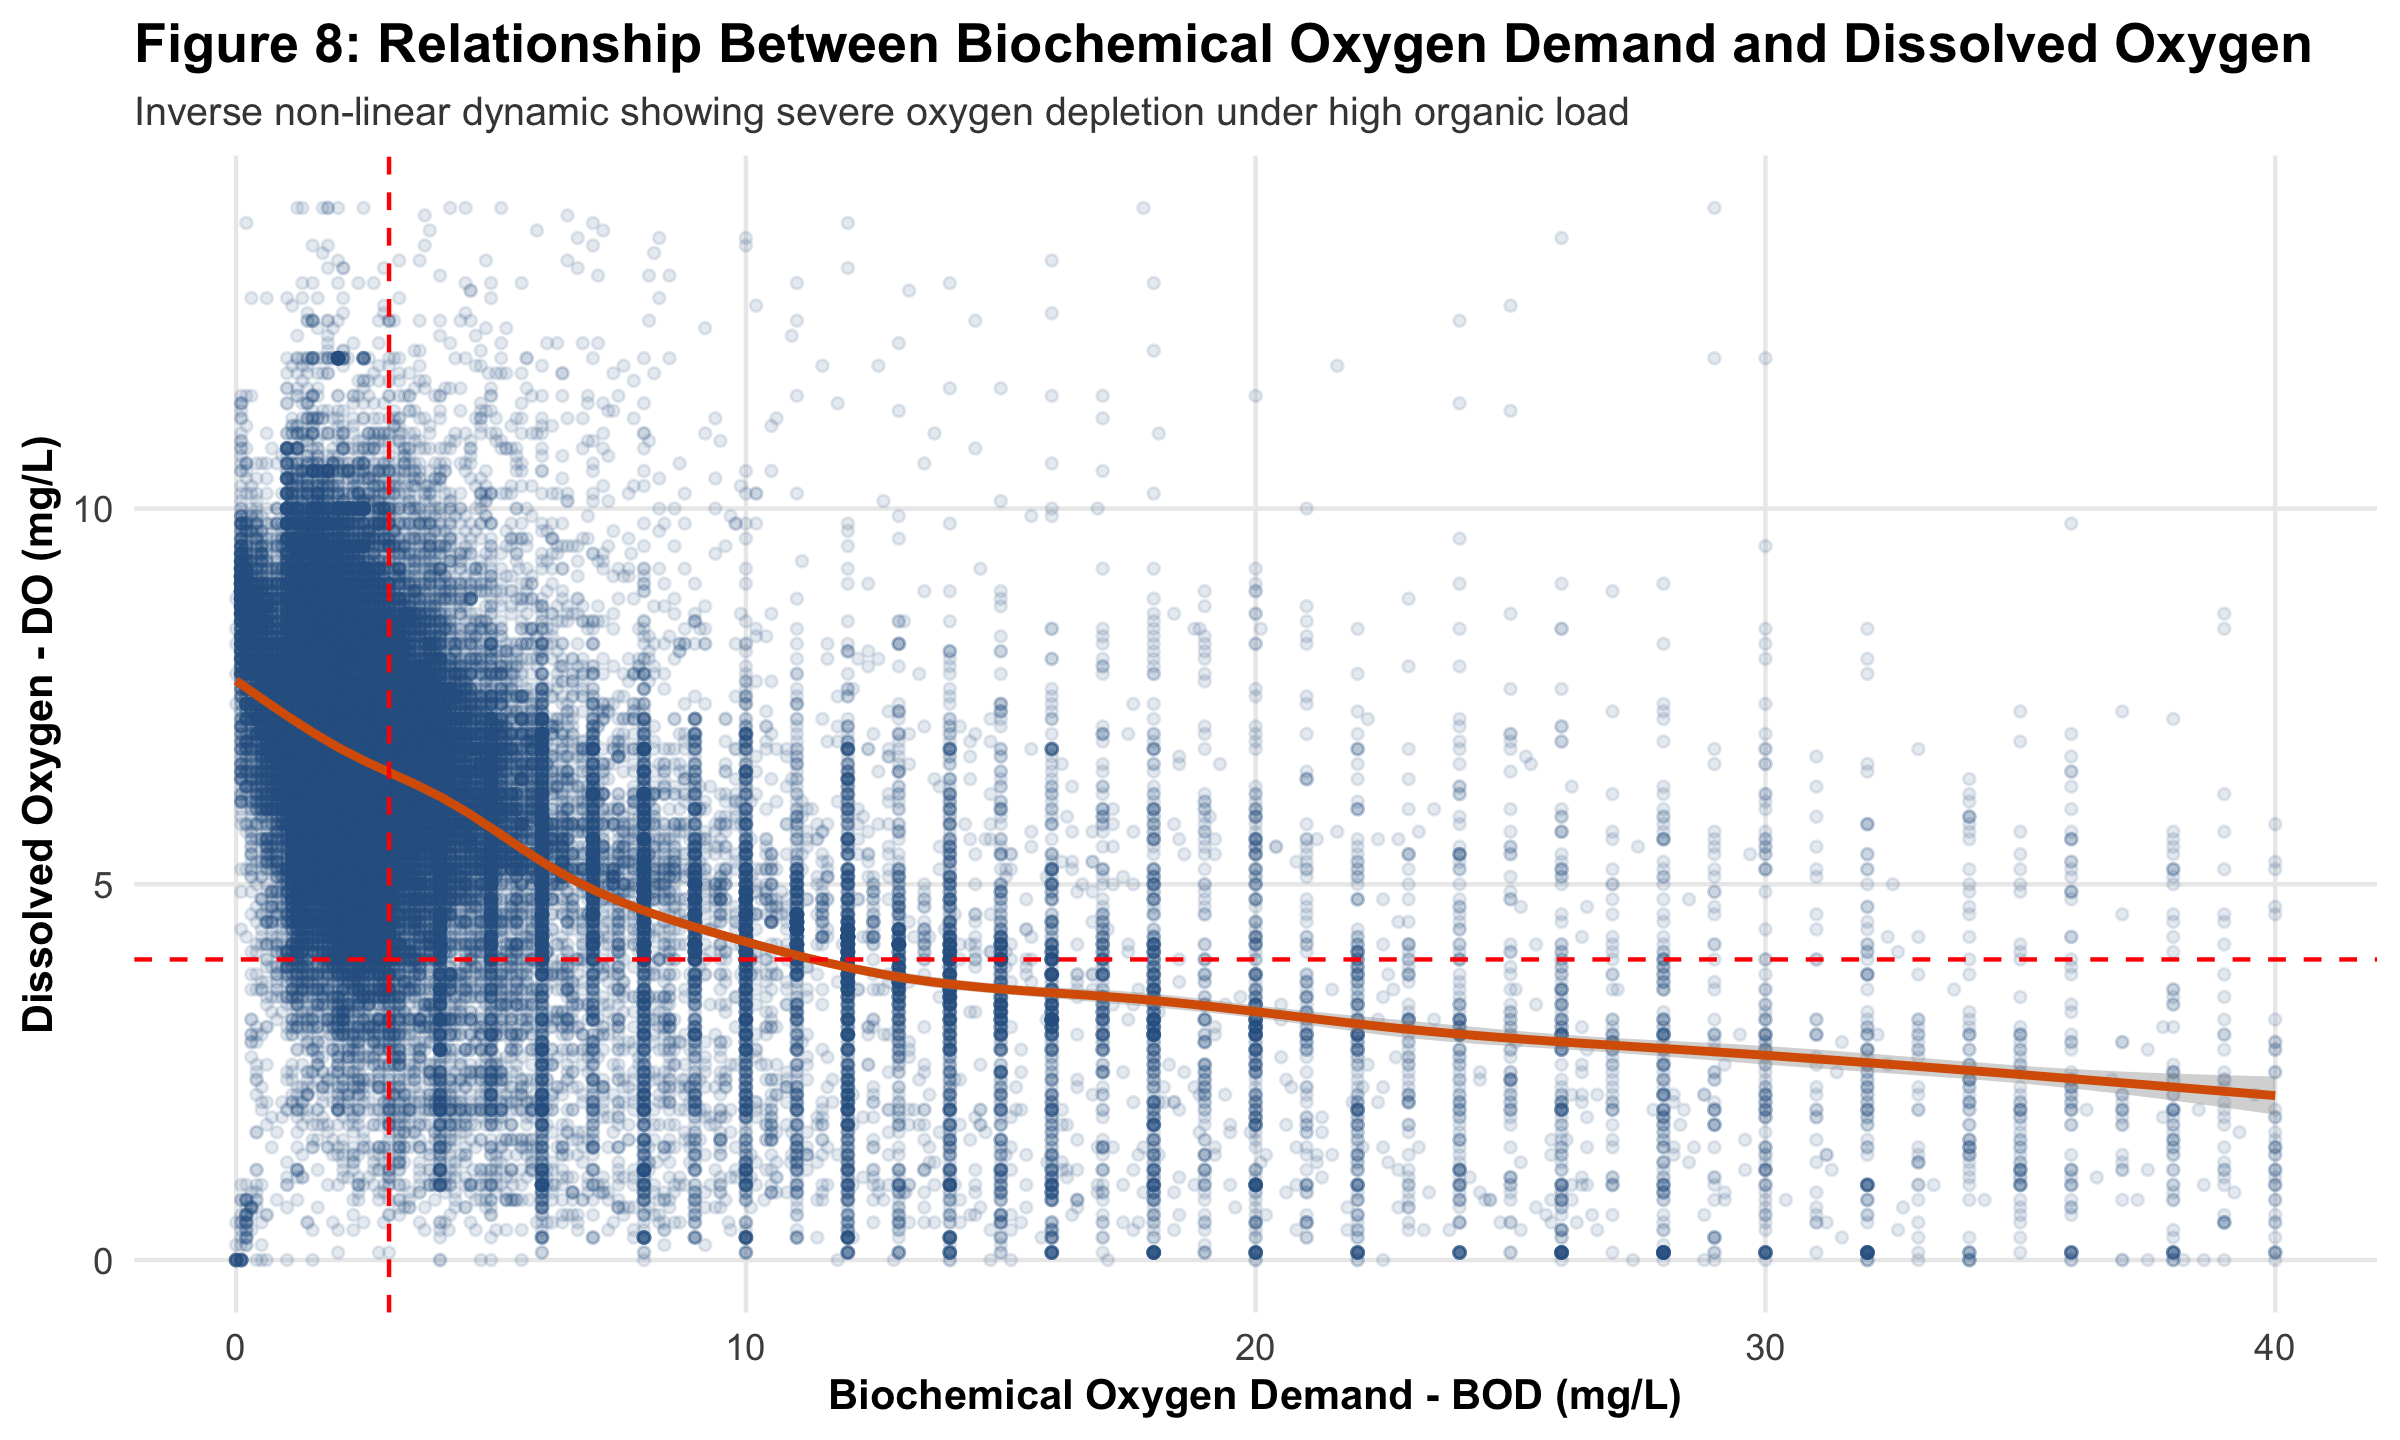
\includegraphics[width=0.85\linewidth]{figures/08_do_vs_bod_relationship} 

}

\caption{Figure: Non-linear Relationship Between BOD and Dissolved Oxygen}\label{fig:fig-do-bod-scatter}
\end{figure}

\emph{Interpretation of BOD vs.~DO Relationship:} The scatter plot shows
the expected inverse non-linear relationship between BOD and DO. In
clean waters where \(\text{BOD} \le 3.0\text{ mg/L}\), DO concentrations
remain healthy (\(6.0–9.0\text{ mg/L}\)). As organic load escalates
(\(\text{BOD} > 10\text{ mg/L}\)), microbial decomposition rapidly
consumes oxygen, driving DO down toward severe hypoxia
(\(< 2.0\text{ mg/L}\)).

\begin{Shaded}
\begin{Highlighting}[]
\NormalTok{knitr}\SpecialCharTok{::}\FunctionTok{include\_graphics}\NormalTok{(}\FunctionTok{file.path}\NormalTok{(FIG\_DIR, }\StringTok{"06\_correlation\_matrix.png"}\NormalTok{))}
\end{Highlighting}
\end{Shaded}

\begin{figure}

{\centering 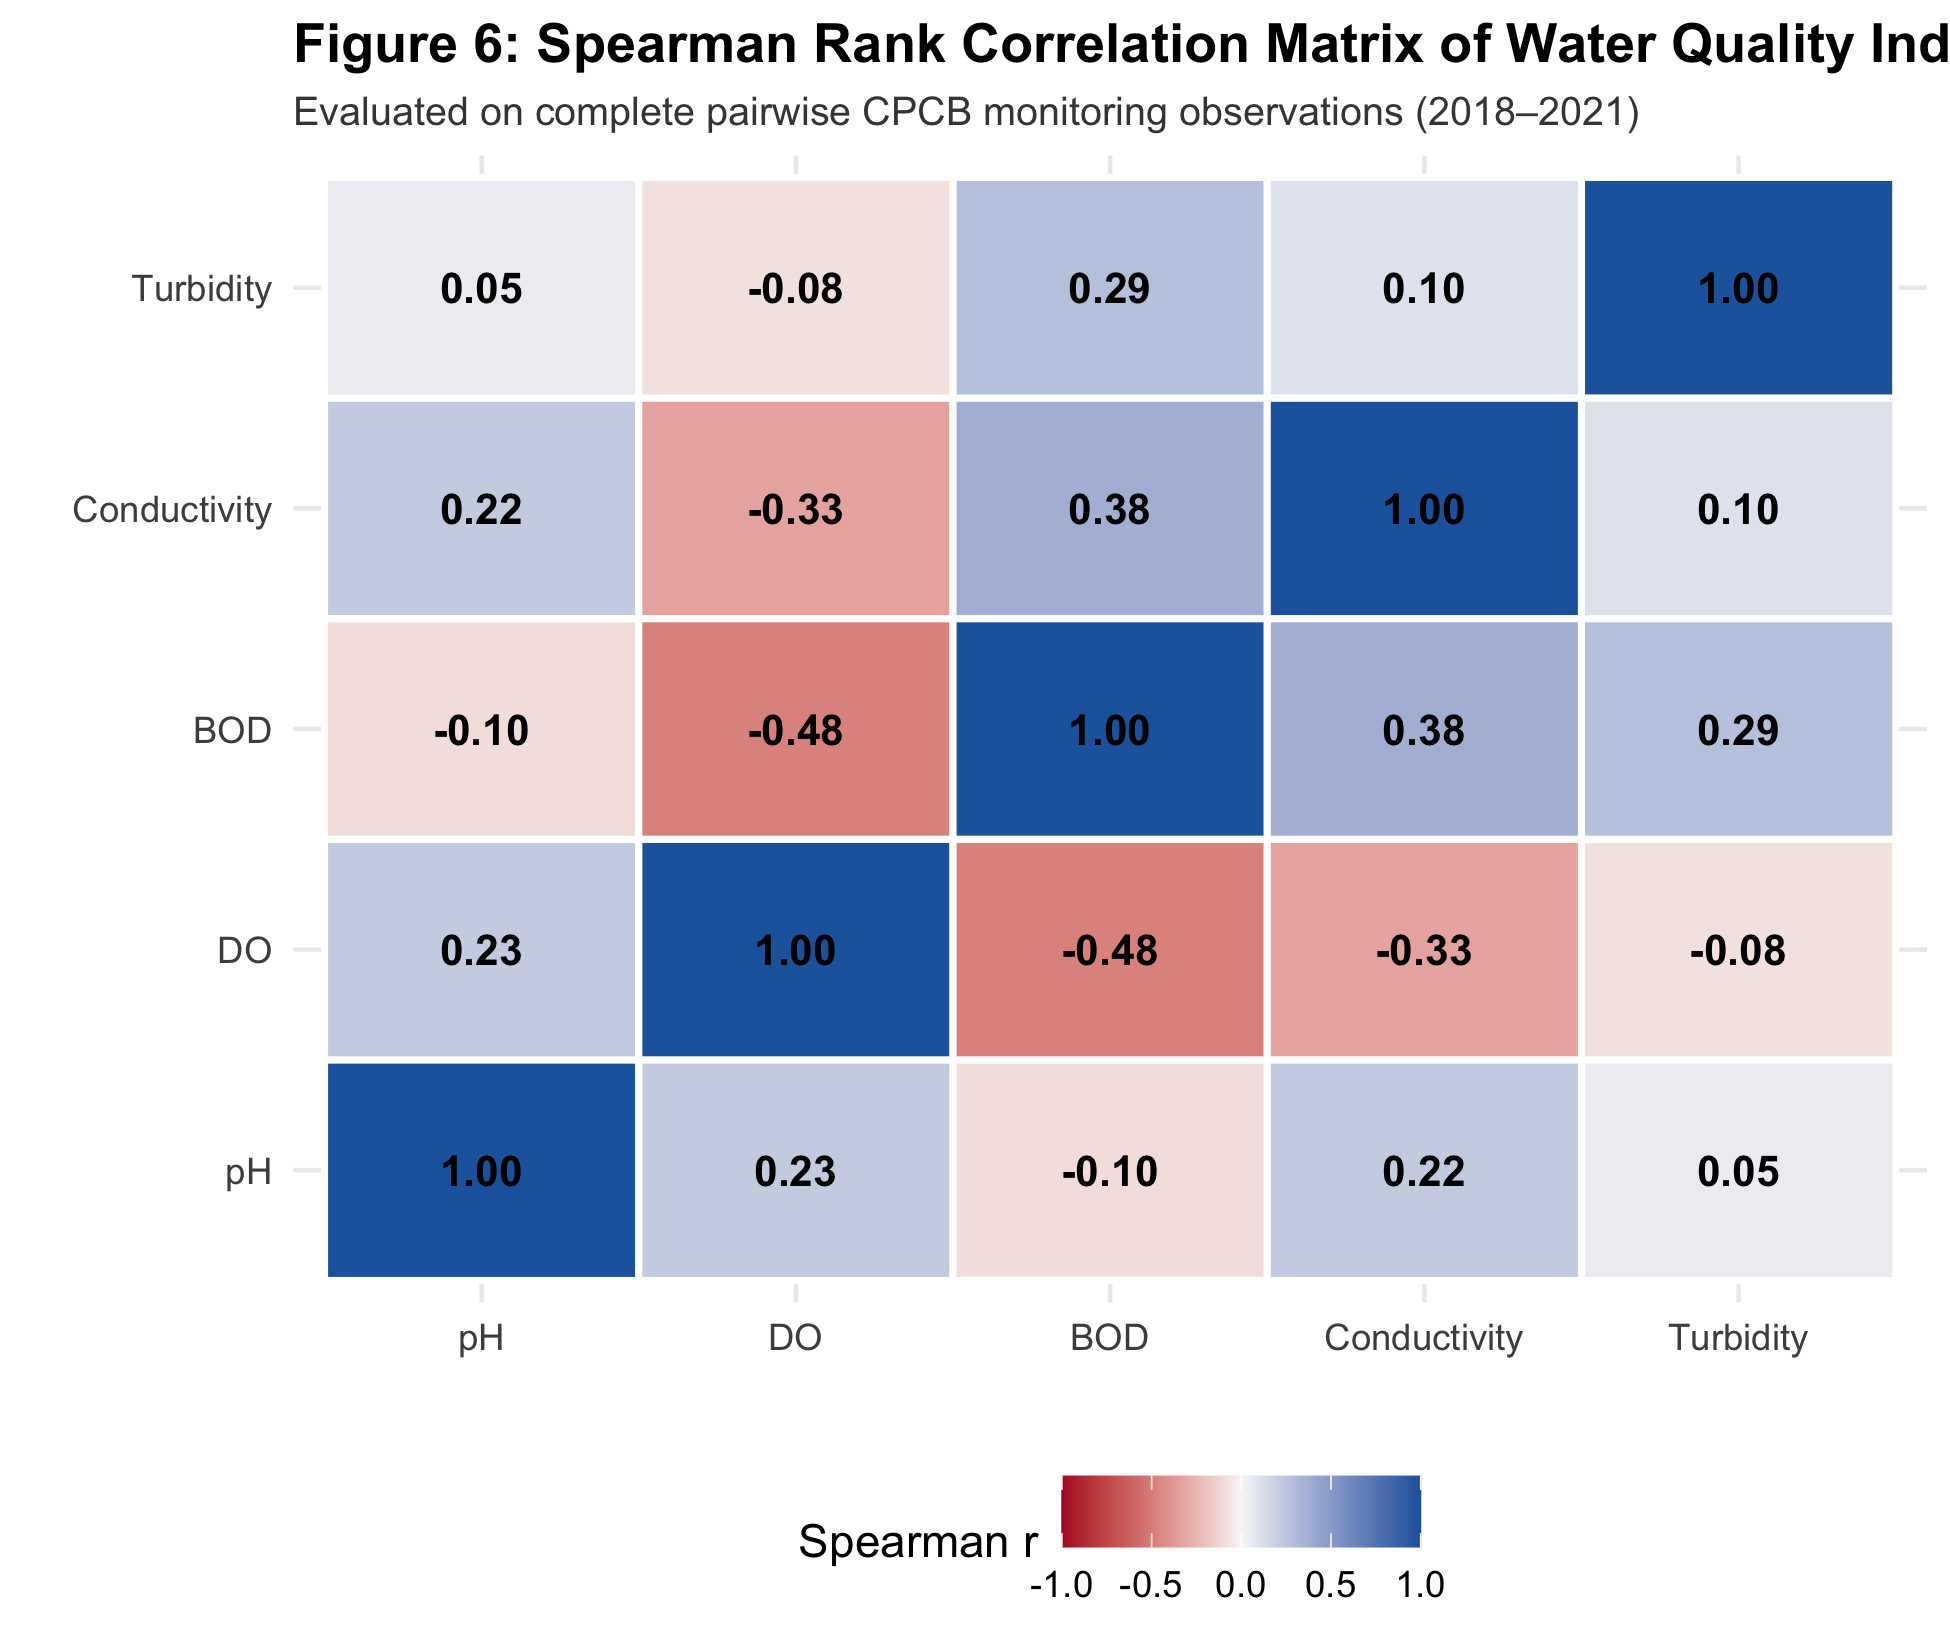
\includegraphics[width=0.75\linewidth]{figures/06_correlation_matrix} 

}

\caption{Figure: Spearman Rank Correlation Matrix of Key Water Quality Indicators}\label{fig:fig-cor-matrix}
\end{figure}

\emph{Interpretation of Correlation Matrix:} Due to skewed
distributions, Spearman's rank correlation (\(\rho\)) was computed: -
\textbf{DO vs.~BOD:} Negative correlation (\(\rho = -0.34\)), confirming
that higher organic loads correspond to oxygen depletion. -
\textbf{Conductivity vs.~DO:} Negative correlation (\(\rho = -0.22\)),
as dissolved salts and wastewater discharge reduce oxygen solubility. -
\textbf{Conductivity vs.~Turbidity:} Positive correlation
(\(\rho = 0.28\)), reflecting simultaneous influx of suspended and
dissolved solids during runoff events.

\begin{center}\rule{0.5\linewidth}{0.5pt}\end{center}

\section{Historical Comparison: Kaggle Baseline vs.~Modern
CPCB}\label{historical-comparison-kaggle-baseline-vs.-modern-cpcb}

\subsection{Methodological Distinctions Between
Datasets}\label{methodological-distinctions-between-datasets}

A central question is whether the historical Kaggle dataset (2003--2014)
can be directly combined with the modern CPCB dataset (2018--2021). As
established in our feasibility assessment, row-level merging is
methodologically invalid for several reasons:

\begin{enumerate}
\def\labelenumi{\arabic{enumi}.}
\tightlist
\item
  \textbf{Temporal Disconnect:} A complete 4-year gap separates the two
  datasets (2014 to 2018).
\item
  \textbf{Aggregation Asymmetry:} Kaggle contains single annual summary
  means per station-year, whereas CPCB contains high-frequency periodic
  event observations.
\item
  \textbf{Spatial Discrepancy:} The CPCB dataset includes full WGS84 GPS
  coordinates for 4,017 stations, while the Kaggle dataset contains zero
  coordinates.
\end{enumerate}

Therefore, we restrict our comparison to \textbf{aggregated state-level
medians} for shared parameters:

\begin{Shaded}
\begin{Highlighting}[]
\CommentTok{\# Load cleaned Kaggle dataset for comparison}
\ControlFlowTok{if}\NormalTok{ (}\SpecialCharTok{!}\FunctionTok{exists}\NormalTok{(}\StringTok{"df\_kag"}\NormalTok{)) \{}
\NormalTok{  df\_kag }\OtherTok{\textless{}{-}} \FunctionTok{read.csv}\NormalTok{(}\FunctionTok{file.path}\NormalTok{(PROC\_DIR, }\StringTok{"kaggle\_water\_quality\_clean.csv"}\NormalTok{), }\AttributeTok{stringsAsFactors =} \ConstantTok{FALSE}\NormalTok{)}
\NormalTok{\}}

\CommentTok{\# State{-}level aggregation for common states with \textgreater{}= 15 historical records}
\NormalTok{k\_agg }\OtherTok{\textless{}{-}}\NormalTok{ df\_kag }\SpecialCharTok{\%\textgreater{}\%} 
  \FunctionTok{filter}\NormalTok{(}\SpecialCharTok{!}\FunctionTok{is.na}\NormalTok{(state), }\SpecialCharTok{!}\FunctionTok{is.na}\NormalTok{(dissolved\_oxygen\_mg\_l)) }\SpecialCharTok{\%\textgreater{}\%} 
  \FunctionTok{group\_by}\NormalTok{(state) }\SpecialCharTok{\%\textgreater{}\%} 
  \FunctionTok{summarise}\NormalTok{(}\AttributeTok{Hist\_Median\_DO =} \FunctionTok{round}\NormalTok{(}\FunctionTok{median}\NormalTok{(dissolved\_oxygen\_mg\_l), }\DecValTok{2}\NormalTok{), }\AttributeTok{Hist\_N =} \FunctionTok{n}\NormalTok{()) }\SpecialCharTok{\%\textgreater{}\%} 
  \FunctionTok{filter}\NormalTok{(Hist\_N }\SpecialCharTok{\textgreater{}=} \DecValTok{15}\NormalTok{)}

\NormalTok{c\_agg }\OtherTok{\textless{}{-}}\NormalTok{ df\_cpcb\_master }\SpecialCharTok{\%\textgreater{}\%} 
  \FunctionTok{filter}\NormalTok{(}\SpecialCharTok{!}\FunctionTok{is.na}\NormalTok{(state), }\SpecialCharTok{!}\FunctionTok{is.na}\NormalTok{(dissolved\_oxygen\_mg\_l)) }\SpecialCharTok{\%\textgreater{}\%} 
  \FunctionTok{group\_by}\NormalTok{(state) }\SpecialCharTok{\%\textgreater{}\%} 
  \FunctionTok{summarise}\NormalTok{(}\AttributeTok{Modern\_Median\_DO =} \FunctionTok{round}\NormalTok{(}\FunctionTok{median}\NormalTok{(dissolved\_oxygen\_mg\_l), }\DecValTok{2}\NormalTok{), }\AttributeTok{Modern\_N =} \FunctionTok{n}\NormalTok{())}

\NormalTok{comp\_table }\OtherTok{\textless{}{-}} \FunctionTok{inner\_join}\NormalTok{(k\_agg, c\_agg, }\AttributeTok{by =} \StringTok{"state"}\NormalTok{) }\SpecialCharTok{\%\textgreater{}\%} 
  \FunctionTok{mutate}\NormalTok{(}\AttributeTok{DO\_Shift =} \FunctionTok{round}\NormalTok{(Modern\_Median\_DO }\SpecialCharTok{{-}}\NormalTok{ Hist\_Median\_DO, }\DecValTok{2}\NormalTok{)) }\SpecialCharTok{\%\textgreater{}\%} 
  \FunctionTok{arrange}\NormalTok{(}\FunctionTok{desc}\NormalTok{(Modern\_N))}

\FunctionTok{kable}\NormalTok{(}\FunctionTok{head}\NormalTok{(comp\_table, }\DecValTok{12}\NormalTok{), }\AttributeTok{caption =} \StringTok{"Table 5: State{-}Level Comparison of Median Dissolved Oxygen (2003–2014 vs. 2018–2021)"}\NormalTok{)}
\end{Highlighting}
\end{Shaded}

\begin{longtable}[]{@{}
  >{\raggedright\arraybackslash}p{(\linewidth - 10\tabcolsep) * \real{0.2297}}
  >{\raggedleft\arraybackslash}p{(\linewidth - 10\tabcolsep) * \real{0.2027}}
  >{\raggedleft\arraybackslash}p{(\linewidth - 10\tabcolsep) * \real{0.0946}}
  >{\raggedleft\arraybackslash}p{(\linewidth - 10\tabcolsep) * \real{0.2297}}
  >{\raggedleft\arraybackslash}p{(\linewidth - 10\tabcolsep) * \real{0.1216}}
  >{\raggedleft\arraybackslash}p{(\linewidth - 10\tabcolsep) * \real{0.1216}}@{}}
\caption{Table 5: State-Level Comparison of Median Dissolved Oxygen
(2003--2014 vs.~2018--2021)}\tabularnewline
\toprule\noalign{}
\begin{minipage}[b]{\linewidth}\raggedright
state
\end{minipage} & \begin{minipage}[b]{\linewidth}\raggedleft
Hist\_Median\_DO
\end{minipage} & \begin{minipage}[b]{\linewidth}\raggedleft
Hist\_N
\end{minipage} & \begin{minipage}[b]{\linewidth}\raggedleft
Modern\_Median\_DO
\end{minipage} & \begin{minipage}[b]{\linewidth}\raggedleft
Modern\_N
\end{minipage} & \begin{minipage}[b]{\linewidth}\raggedleft
DO\_Shift
\end{minipage} \\
\midrule\noalign{}
\endfirsthead
\toprule\noalign{}
\begin{minipage}[b]{\linewidth}\raggedright
state
\end{minipage} & \begin{minipage}[b]{\linewidth}\raggedleft
Hist\_Median\_DO
\end{minipage} & \begin{minipage}[b]{\linewidth}\raggedleft
Hist\_N
\end{minipage} & \begin{minipage}[b]{\linewidth}\raggedleft
Modern\_Median\_DO
\end{minipage} & \begin{minipage}[b]{\linewidth}\raggedleft
Modern\_N
\end{minipage} & \begin{minipage}[b]{\linewidth}\raggedleft
DO\_Shift
\end{minipage} \\
\midrule\noalign{}
\endhead
\bottomrule\noalign{}
\endlastfoot
Karnataka & 6.95 & 22 & 6.3 & 10009 & -0.65 \\
Odisha & 7.40 & 62 & 7.3 & 7215 & -0.10 \\
Maharashtra & 6.70 & 184 & 5.9 & 5400 & -0.80 \\
Himachal Pradesh & 7.15 & 26 & 8.4 & 5237 & 1.25 \\
Kerala & 6.70 & 442 & 6.7 & 4457 & 0.00 \\
Gujarat & 6.00 & 76 & 6.7 & 3409 & 0.70 \\
Meghalaya & 7.30 & 153 & 7.2 & 2846 & -0.10 \\
Tamil Nadu & 6.90 & 92 & 6.4 & 2607 & -0.50 \\
Mizoram & 6.90 & 24 & 6.5 & 2379 & -0.40 \\
Tripura & 6.35 & 30 & 6.2 & 2332 & -0.15 \\
Goa & 6.70 & 155 & 6.5 & 2277 & -0.20 \\
Punjab & 5.10 & 119 & 7.0 & 2152 & 1.90 \\
\end{longtable}

\begin{Shaded}
\begin{Highlighting}[]
\NormalTok{knitr}\SpecialCharTok{::}\FunctionTok{include\_graphics}\NormalTok{(}\FunctionTok{file.path}\NormalTok{(FIG\_DIR, }\StringTok{"07\_decadal\_historical\_comparison.png"}\NormalTok{))}
\end{Highlighting}
\end{Shaded}

\begin{figure}

{\centering 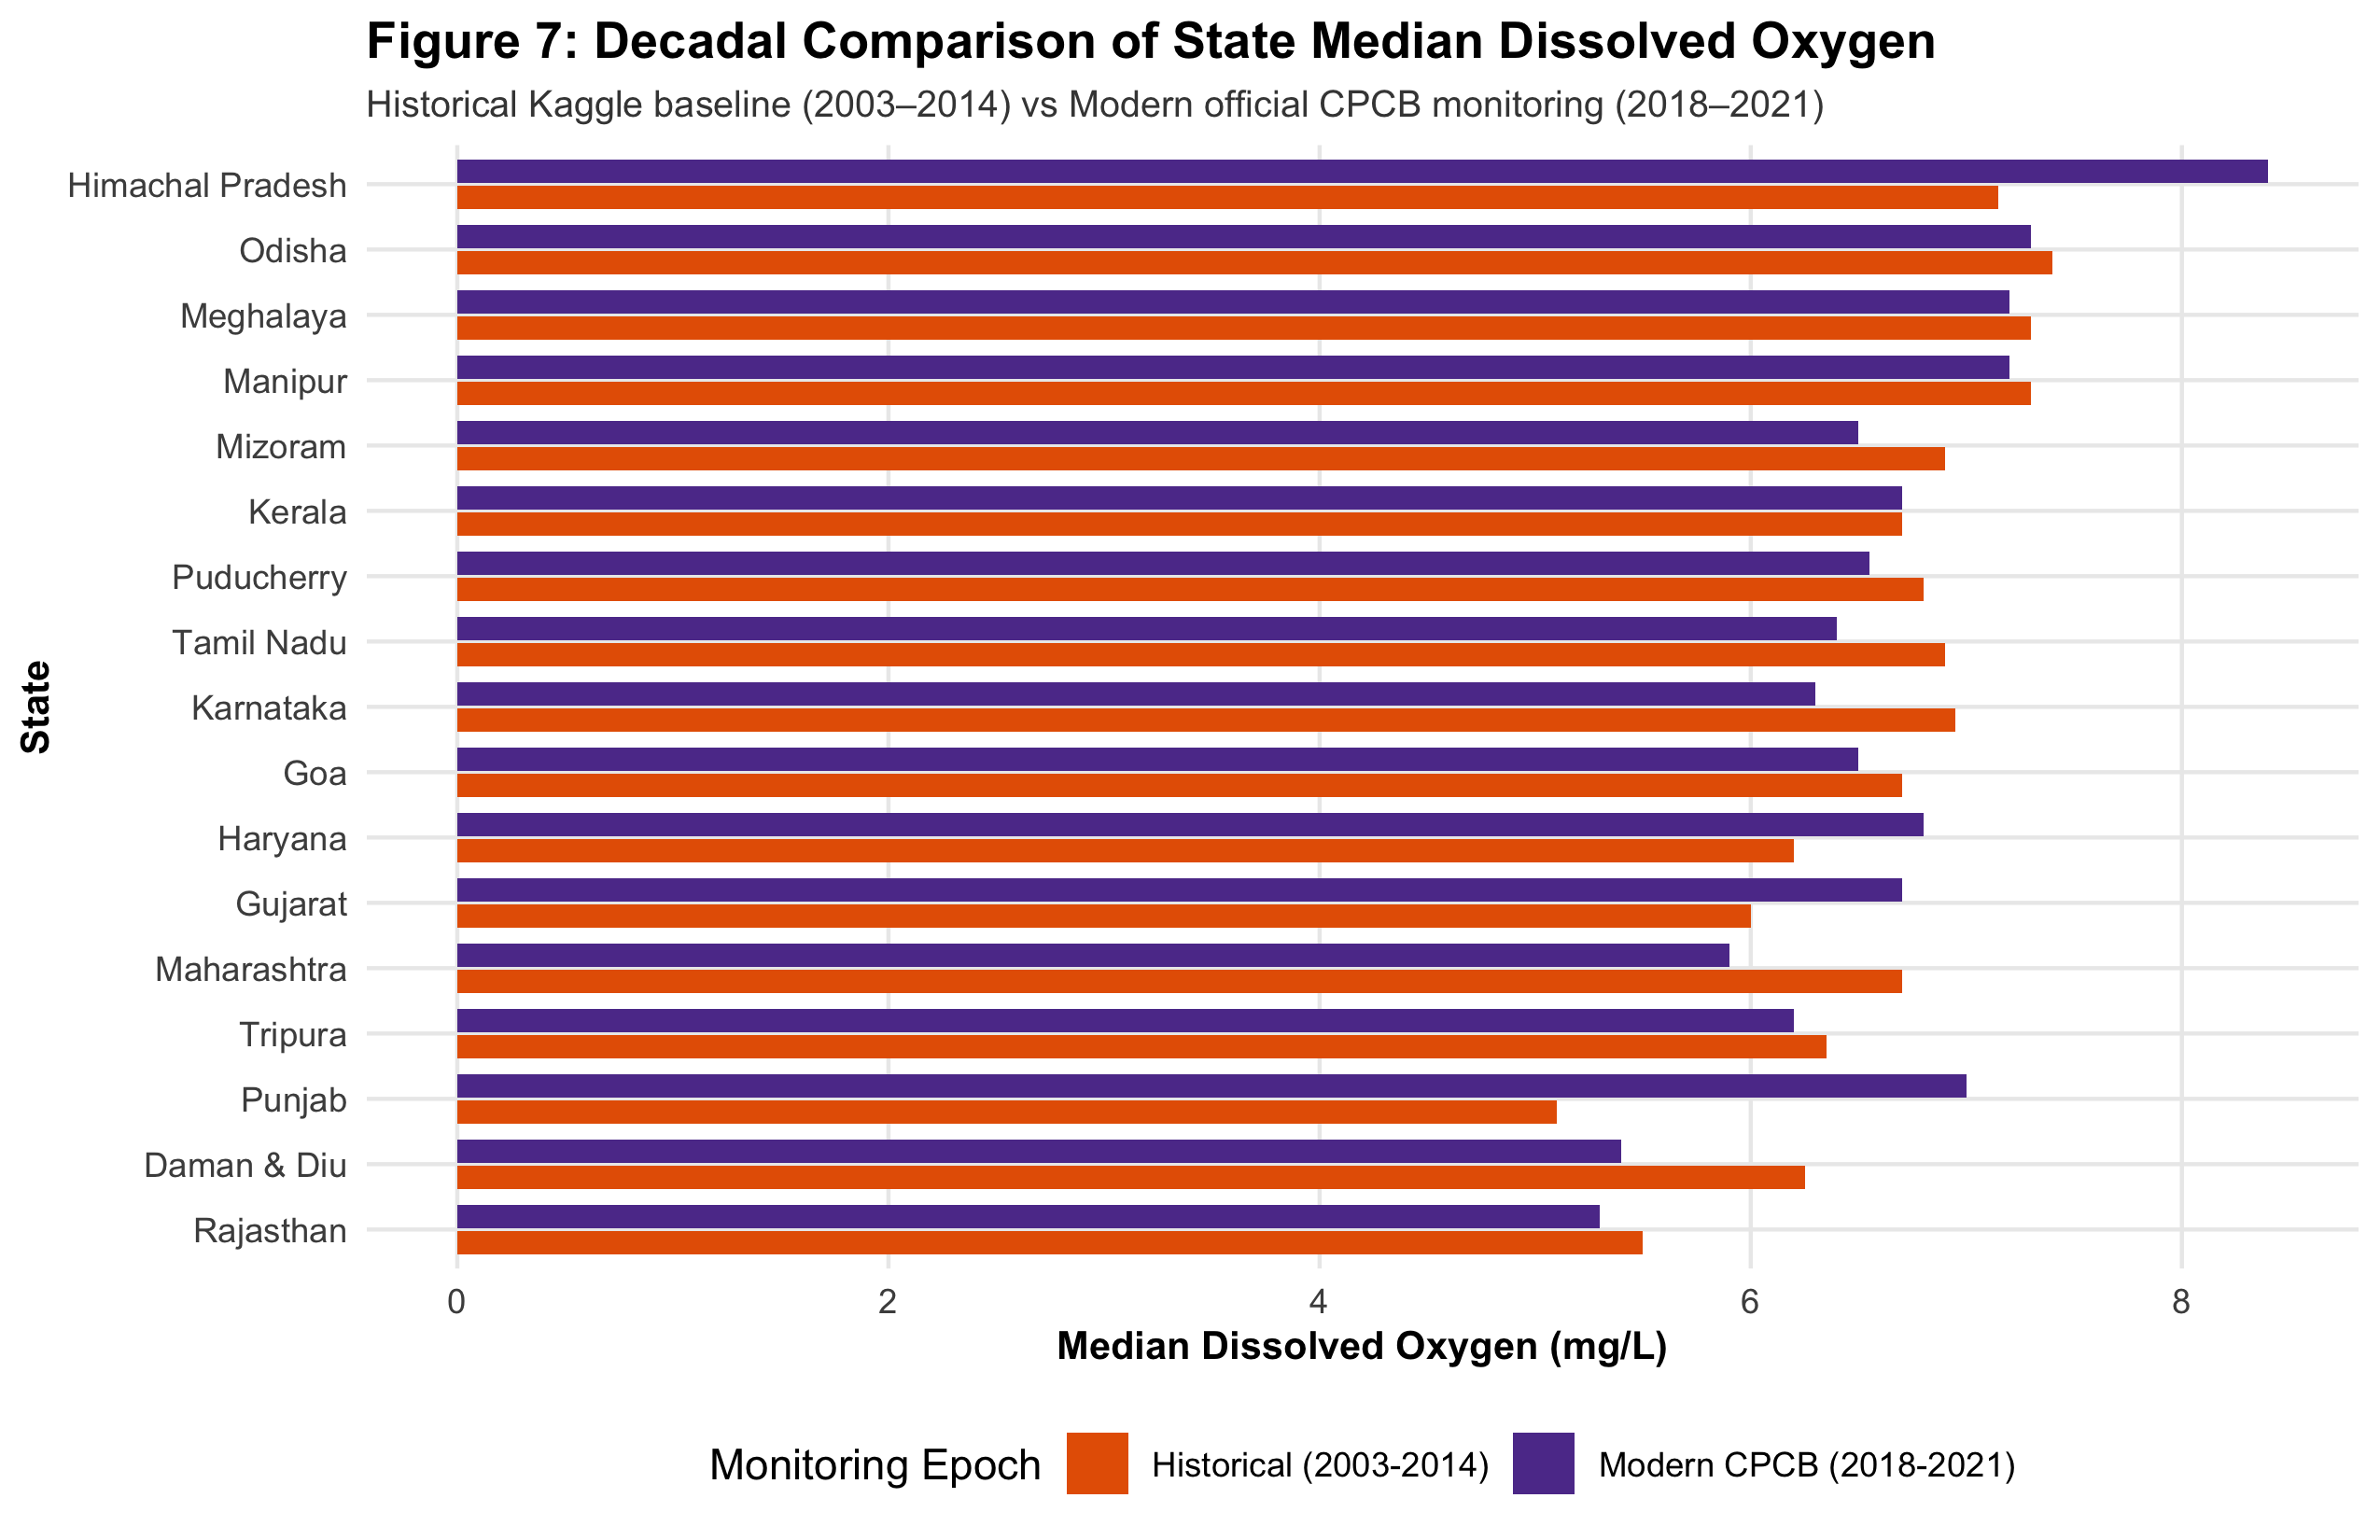
\includegraphics[width=0.85\linewidth]{figures/07_decadal_historical_comparison} 

}

\caption{Figure: Decadal Comparison of State Median Dissolved Oxygen (Historical vs Modern)}\label{fig:fig-historical-comp}
\end{figure}

\emph{Interpretation of Historical Comparison:} Comparing state-level
medians reveals stability in high-quality states (e.g., Kerala, Goa, and
Himachal Pradesh maintain median \(\text{DO} \ge 6.5\text{ mg/L}\)). In
heavily industrialized states (e.g., Gujarat and Maharashtra), median DO
values show slight increases, but also wider variance.

Importantly, these observed differences reflect not only changes in
underlying water quality, but also major expansions in the CPCB
monitoring network (which grew from roughly 321 stations in the Kaggle
era to over 4,000 georeferenced stations by 2018--2021). Consequently,
differences should be interpreted as \textbf{descriptive baseline
comparisons} rather than definitive proof of nationwide environmental
trends.

\begin{center}\rule{0.5\linewidth}{0.5pt}\end{center}

\section{Conclusion}\label{conclusion}

\subsection{Summary of Data Science
Workflow}\label{summary-of-data-science-workflow}

This investigation completed a full end-to-end data science workflow on
surface water quality monitoring data from India:

\begin{enumerate}
\def\labelenumi{\arabic{enumi}.}
\tightlist
\item
  \textbf{Inspection \& Profiling:} Examined 315 official CPCB CSV files
  (311,379 observations) and 1 Kaggle dataset (1,991 rows). Diagnosed
  encoding mismatches (\texttt{latin1}), OCR header defects, and
  identified a misclassified biological file in the chemical directory.
\item
  \textbf{Data Cleaning:} Implemented reproducible cleaning pipelines in
  R, removing full duplicates, normalizing missingness markers,
  recovering misaligned state names, and replacing impossible values
  (such as 89 Kaggle \(\text{pH} > 14\) and 11 CPCB
  \(\text{DO} > 25\text{ mg/L}\)) with \texttt{NA} rather than
  discarding whole records.
\item
  \textbf{Exploratory Data Analysis:} Profiled empirical distributions,
  mapped station coordinates across India, and quantified seasonal
  dilution effects.
\item
  \textbf{Hypothesis Testing:} Confirmed statistically significant
  state-level differences in BOD (\(\chi^2 = 11,725.65\), \(p < 0.001\))
  and verified seasonal DO variations between pre-monsoon and monsoon
  periods (\(p = 5.48 \times 10^{-24}\)).
\item
  \textbf{Decadal Comparison:} Conducted a state-level aggregated
  comparison between historical (2003--2014) and modern (2018--2021)
  monitoring data, avoiding flawed row-level merging.
\end{enumerate}

\subsection{Key Empirical Findings}\label{key-empirical-findings}

\begin{itemize}
\tightlist
\item
  \textbf{Dissolved Oxygen Compliance:} Modern CPCB monitoring indicates
  an overall median DO of \(6.80\text{ mg/L}\), with \(90.8\%\) of
  records meeting the Class C standard (\(\ge 4.0\text{ mg/L}\)).
\item
  \textbf{Organic Pollution Pockets:} BOD exhibits severe right-skewness
  (\(Median = 2.30\text{ mg/L}\), \(Mean = 5.76\text{ mg/L}\),
  \(Max = 1,315\text{ mg/L}\)), reflecting localized industrial and
  domestic sewage inputs.
\item
  \textbf{Monsoon Dilution Effect:} High monsoon discharge reduces
  median BOD and increases re-aeration compared to pre-monsoon summer
  lows.
\item
  \textbf{Oxygen Depletion Dynamics:} Non-linear modeling confirms rapid
  oxygen depletion once BOD exceeds \(5–10\text{ mg/L}\).
\end{itemize}

\subsection{Project Limitations}\label{project-limitations}

\begin{itemize}
\tightlist
\item
  \textbf{Parameter Missingness:} Trace heavy metals (arsenic, lead,
  cadmium) exhibited missingness rates exceeding \(60\%\), limiting
  longitudinal heavy metal modeling.
\item
  \textbf{Network Expansion:} The modern CPCB network contains over 10
  times more monitoring stations than the historical Kaggle dataset,
  meaning temporal shifts reflect both monitoring coverage expansion and
  environmental changes.
\item
  \textbf{Monitoring Frequency:} While CPCB data provides periodic event
  timestamps, sampling intervals vary between monthly and quarterly
  across states.
\end{itemize}


\end{document}
